\documentclass[a4paper,10pt]{book}
\usepackage[utf8]{inputenc}

\usepackage[utf8]{inputenc}
\usepackage[english]{babel} %francais, polish, spanish, ...
\usepackage[T1]{fontenc}


\usepackage{amsfonts}
\usepackage{amsmath}
\usepackage{amssymb}
\usepackage{graphicx}
\usepackage{dcolumn}
\usepackage{latexsym}
\usepackage{hyperref}
\usepackage{bm}
\usepackage[english]{babel}
\usepackage{xcolor}





\usepackage{lmodern} %Type1-font for non-english texts and characters
\usepackage{amsthm}
\usepackage{amsfonts}
\usepackage{float}
\usepackage{ mathrsfs }


\usepackage[utf8]{inputenc}
\usepackage[T1]{fontenc}
\usepackage{textcomp}
\usepackage{gensymb}
\usepackage{subcaption}

\usepackage{enumitem}


\def \ep{\epsilon}

\newtheorem{lemma}{Lema}
\newtheorem{ejemplo}{Ejemplo}
\newtheorem{propiedades}{Propiedades}
\newtheorem{definition}{Definición}
\newtheorem{theorem}{Teorema}
\newtheorem{proposition}{Proposición}

\newcommand{\rotin}{\mathbin{\rotatebox[origin=c]{270}{$\in$}}}
\newcommand{\rotnotin}{\mathbin{\rotatebox[origin=c]{270}{$\notin$}}}
\newcommand{\roteq}{\mathbin{\rotatebox[origin=c]{270}{$=$}}}




\begin{document}


\section{Introducci\'on}
Queremos buscar los m\'inimos del siguiente problema:$\mathscr{L}$ es un operador lineal
$\mathscr{L} U=f$.   Si definimos
\[A(U,v)=\iint_{\Omega} \mathscr{L} U v dx \] 
$A$ es tal que $A(U,v)\geq \alpha {|| U ||}^2$.  $U_0$ es m\'inimo de 
\[A(U,U)-2 (f,U) \]
donde 
\[(f,U)=\iint_{\Omega} f U dx.\]
entonces a $U_0$ se le llama la soluci\'on generalizada de $\mathscr{L} u=f$. El operador $\mathscr{L}$ puede ser 
por ejemplo la  biarm\'onica $\Delta^2$.
si
\[\iint_{\Omega} \mathscr{L} U\varphi dx =\iint_{\Omega} f \varphi dx  \]
para todo $\varphi \in C_0^\infty$, entonces definimos el operador autoadjunto como 
\[\iint_{\Omega} U \mathscr{L}^{*} \varphi \]
Ejemplos f\'isicos de este operador son 
la membrana el\'astica y el campo electrost\'atico. En cualquiera de estos casos
vemos que la energ\'ia almacenada por el campo se puede escribir de la forma
\[I(U)=\iint_{\Omega} |\nabla U |^2 dx \]
El problema lo plantearemos como : encontrar $u$  que minimiza $I(U)$ con $U|_{\partial \Omega}=f$ .
Primero veremos que el minimizar la energia es equivalente a encontrar la soluci\'on al problema 
del laplaciano con valor en la frontera. Sea $v$ tal que $v|_{\partial \Omega}=f$ y sea
$h=v-U$ entonces $h|_{\partial \Omega}=0$. Ahora
\[I(v)= I(U+h)=  \iint_{\Omega} (U_x +h_x)^2+(U_y+h_y)^2  \]
el teorema de Green 
\[
\iint_\Omega U\Delta v = - \iint_\Omega \nabla U \cdot \nabla v + \int_{\partial \Omega} U \frac{\partial v}{\partial n}
\]
entonces

\[I(v)=I(U)+I(h)-2\iint_{\Omega} h \Delta U  \] 
donde usamos el hecho que $h$ vale cero en la frontera. Si el laplaciano de $U$ es positivo en un punto $(x_0,y_0)$
entonces ser\'a positivo en una vecindad de $(x_0,y_0)$.  Tomamos $h<0$ fuera de una vecindad de $(x_0,y_0)$, entonces se tiene que 
\[I(U+h)\geq I(U)\].

Ahora si tomamos
$h>0$ en la vecindad y cero fuera y tal que $\iint_{\Omega} |\nabla h|^2 =1$   entonces
\[I(U+\epsilon h)-I(U)= \epsilon^2-2\epsilon \iint_{\Omega} h \Delta U <0\]
si $ \epsilon$ es peque\~no, lo que contradice que $I(U)$ sea m\'inimo. Lo que implica que
$\Delta U\leq 0$ y por lo tanto $\Delta U=0$ y por lo tanto $u$ m\'inimo de $I(U)$  con $U|_{\partial \Omega} =f$ es necesario
y suficiente para que $\Delta U=0$ en $\Omega$ y $U|_{\partial \Omega}=f$.

\subsection*{\underline{La soluci\'on es \'unica}.}

Si $u_1$ y $u_2$ son soluciones, $h=u_1-u_2$ entonces
\[I(u_1)=I(u_2+h)=I(u_2)+I(h)\]
y como $I(u_1)=I(u_2)$ implica que $I(h)=0$ y por lo tanto $\nabla h=0$ y por lo tanto 
$h=cte=0$ en $\partial \Omega$.

\subsection*{\underline{Principio de Dirichlet}.}
Tenemos las siguientes preguntas:
\begin{enumerate}
 \item \textquestiondown Existe una soluci\'on de $\Delta U=0$ 
en $\Omega$, talque $U|_{\partial \Omega}=f$ ?.\textquestiondown Que tipo de solución es ?
Acaso $U\in C^2 (\Omega) \cap C^0 (\bar{\Omega})$ donde la barra indica la cerradura de $\Omega$.
Si es \'unica  $h=u_1-u_2$ implica $\Delta h=0$ y $h|_{\partial \Omega} =0$ implica el principio
del m\'aximo que a su vez implica que $h=0$.

\item \textquestiondown Existe un m\'inimo ?
\item \textquestiondown Como se calcula el m\'inimo $I(U)=\iint_{\Omega}  |\nabla U|^2 $.
\item Si existe el m\'inimo $u$ implica acaso que $U\in C^2 (\Omega) \cap C^0 (\bar{\Omega})$ implica 
acaso que la energ\'ia es finita ?
\end{enumerate}

Ilustraremos estas preguntas con un ejemplo. 

\subsection*{1)\underline{Ejemplo de Hadamard}.}

Sea $\Omega $ un disco unitario. Consideremos la funci\'on sobre la frontera del 
disco unitario parametrizada por el \'angulo $\theta\in [0,2\pi]$

\begin{equation}
\label{hadamard}
  f(\theta)=\sum\limits_{n=1}^{\infty} \frac{cos(2^{2n} \theta)}{2^n}
\end{equation}

Como $|f(\theta)|\leq \sum\limits \frac{1}{2^n} =1$ (como puede verse de sumar la serie geom\'etrica con $r=1/2$),
entonces al serie es absolutamente convergente. Que implica que $f(\theta)$ es continua.
sea 
\[u(x,y)=u(\rho,\theta)=\sum\limits_{n=1}^{\infty}  \rho ^{2 ^{2n} } \frac{\cos(2^{2n} \theta)}{2^n}\]
esta funci\'on cumple que $u|_{\partial \Omega}=f(\theta)$  y $|u(x,y)|\leq 1$ y
\[u(x,y)= Re \left( \sum\limits_{n=1}^\infty \frac{z^{2^{n}} }{2^n}\right) \]
es una funci\'on anal\'itica para $|z|<1$  lo que implica que $u$ es arm\'onica. Ahora para pasar a coordenadas
polares usamos el hecho que 
\[u_x=u_\rho \cos \theta - u_{\theta} \frac{\sin \theta}{\rho} \]
\[u_y=u_\rho \sin \theta  + u_{\theta} \frac{\cos \theta}{\rho}.\]

La energ\'ia se calcula como
\[ I(u)= \iint_{\Omega} (u_x^2+u_y^2)= \int_0^1 \int_0^{2\pi} \left( u_{\rho} ^{2} + \frac{u_\theta ^2 }{\rho^2} \right) \rho d\rho d\theta
\]
Sustituyendo se tendr\'ia que

\[ I(u)= \int_0^1 \int_0^{2\pi} \left( 
 \sum\limits_{n=1}^{\infty}  2^{2n} \frac{\rho ^{2 ^{2n}-1 } }{2^n} \frac{\cos(2^{2n} \theta)}{2^n} \right)^2+
\]
\[
 \left( 
 \sum\limits_{n=1}^{\infty} (-) 2^{2n} \frac{\rho ^{2 ^{2n} } }{2^n} \frac{\sin(2^{2n} \theta)}{2^n} \right)^2 \frac{1}{\rho^2} \rho 
d\rho d\theta.
\]

Como los dobles productos de senos y cosenos son cero, entonces

\[I(u)=\left.2\pi \sum\limits_{n=1}^{\infty} \frac{2^{2n}}{2^{2n+1} } \rho^{2^{2n+1}}\right|_0^1=\pi \sum\limits_{n=1}^{\infty} \rho^{2n+1}=\infty.\]

Moraleja, tengo que trabajar con una clase m\'as chica de funciones en la frontera. Esta clase ser\'a $f|_{\partial \Omega}$ y
si definimos los siguientes espacios, entonces

\[ L^2 (S^1)=\left\lbrace g(\theta)=\sum\limits_{n=-\infty}^{\infty} a_n e^{i n \theta } \in Re \Leftrightarrow
 a_{-n}=\bar{a}_n \right\rbrace
\]
con 
\[\sum\limits |a_n|^2 =\int_{0}^{2\pi} |g(\theta)|^2 d\theta < \infty \]

Podemos definir los espacios de funciones
\[H^{\alpha}(S^1)=\left\lbrace  g(\theta) = \sum\limits_{-\infty}^{\infty} a_n e^{in\theta}, a_{-n}=\bar{a}_n, \sum\limits_{-\infty}^{\infty} |a_n|^2 n^{2\alpha} <\infty  \right\rbrace.
\]
en particular
\[H^1(S^1)=\left\lbrace g: \sum\limits_{n=-\infty}^{\infty} | a_n|^2 n^2 =\int_0^{2\pi} |g'(\theta)|^2 d\theta \right\rbrace < \infty \] 
Para ver a que espacio de funciones corresponde la funci\'on  del ejemplo de Hadamard (\ref{hadamard}) vemos que
\[\sum\limits_{-\infty}^{\infty} |a_n|^2 n^{2\alpha} =\sum\limits_{n=-\infty}^{\infty} \left(\frac{1}{2^n} \right)^2 (2^{2n} )^{2\alpha} =\sum\limits_{n=-\infty}^{\infty} \frac{1}{2^{2n(1-2\alpha)}} \] 
que ser\'a menor que infinito si $\alpha <1/2$  y la serie converge uniformenente. Si $\alpha\geq 1/2$ tenemos una
suma infinita y por lo tanto $f(\theta)\in H^{\alpha}(S^{1} )$ con $\alpha<1/2$ .
Se puede probar que si $f(\theta)\in H^{\alpha}(S^1)$, $\alpha\geq 1/2$ entonces existe
$u$ tal que $u|_{\rho =1}=f$ y $I(u)<\infty$ . (teorema de traza, adem\'as $f$ es continua)

\subsection*{2)\underline{Tipo de soluciones}.}

Sea $f|_{\partial \Omega}$ tal que exista $u_0 \in C^2(\Omega) \cap  C^0(\bar{\Omega}) $, $u_0|_{\partial \Omega}=1$ y $I(u_0)< \infty$.
Sea $u$ talque $\nabla^2 u=0$ , $u\in C^2(\Omega)\cap C^0(\bar{\Omega})$, $I(u)<\infty$, $u|_{\partial \Omega}=f$ sea 
$h=u-u_0$ implica $h \in C^2(\Omega) \cap  C^0(\bar{\Omega})$, $\Delta h=\Delta u-\Delta u_0=-\Delta u_0=g$  es continua. 

Sea 
\[J(k)=\iint_\Omega| \nabla k|^2  + 2\iint_\Omega gk \]
para $k\in C^2 (\Omega)\cap C^0(\bar{\Omega}) $, $k|_{\partial \Omega}=0$ , $I(k)<\infty$. Si definimos

\[J(h)=I(h)+2 \iint_\Omega \Delta h h  = I(h) -2\iint_\Omega | \nabla h |^2 = -I(h)\]
donde hemos utilizado la identidad de Green. Ahora 
\[J(h+k)= I(h+k)+2\iint (h+k)g  \]
\[J(h+k)= I(h)+I(k) -2 \iint k \Delta h+2\iint  (h+k)g \]
\[J(h+k)=J(h) +I(k)+2 \iint_\Omega( g-\Delta h )k \]
cuando $g-\Delta h =0$ da el m\'inimo  de $J(k)$. Alrev\'es,  si $h$ tiene esas propiedades y $J(h)$ es
m\'inimo entonces $\Delta h=g$ en $\Omega$. Entonces tenemos que si definimos el espacio de funciones
\[E=\left\lbrace k\in C^2 (\Omega) \cap C^0(\bar{\Omega} ), k|_{\partial \Omega}=0 \right\rbrace, I(k)<\infty\]
entonces $  \underset{E}{min} J(k)$  es una condici\'on necesaria y suficiente para que $h$ 
sea soluci\'on de la ecuaci\'on si $\Delta h=g$ y como se vi\'o se tiene que

\begin{enumerate}
\item $J(h)=-I(h)$
\item $J(h+k)= J(k)+I(k)$
\item $J(k)\geq I(k)-2\iint_\Omega |g||k| \geq I(k) - \epsilon \iint_\Omega k^2 -\frac{1}{\epsilon} \iint_\Omega g^2 $ \\
donde en $3)$ se utiliz\'o el hecho que si $a,b$ son dos n\'umeros cualesquiera entonces siempre se tiene
que  $2ab\leq \epsilon a^2 +\frac{1}{\epsilon} b^2 $ (teorema del binomio) . Si $|k|=0$ en $\partial\Omega$ entonces el lema de Poincar\'e
nos da que 
\[ \iint_\Omega k^2 \leq \kappa \iint_\Omega |\nabla k|^2\]
donde tomando  $\epsilon=1/\kappa$ tenemos que
\[J(k)\geq -\kappa \iint_\Omega g^2 \]
es decir $J$ es acotado por abajo.

\item Si existe el minimo $k\in E$ ¿aproxima a $h$?

sean $w_1,w_2,....\in E$. "linealmente independientes", tal que cualquier $K$ en $E$ 
es "aproximado" por una combinación finita de las $w$'s
si $\Delta h = g$ y $h|_{\partial \Omega} = 0$

Sean $E_N= \{ \sum\limits_{1}{N} a_i w_i \}$ tiene dimension $N$ $E_N \rightarrow\{ a_1,...,a_N\}$

\[
J_N(a_1,...,a_n) = J |_{E_N} = \iint |\nabla \sum\limits a_i w_i |^2 + 2g \sum\limits a_i w_i 
\]
\[= \iint \sum\limits_{i,j =1}^N a_i a_j \nabla w_i\cdot w_j + 2 \sum\limits_{i}^N a_i g w_i = \text{ polinomio de grado 2 en } a_1,...a_n\]
\[
J_N\geq -k \iint g^2  \Rightarrow \text{ hay un mínimo}
\]

dado por $\frac{\partial J_N }{\partial a_i} = 0$

\[
\frac{\partial J_N }{\partial a_i} = 2 \iint \left(  \sum\limits_{j=1}^M a_j \nabla w_i \cdot \nabla w_j + g w_i \right) = 0 \;\; i=1,...,N
\]

Sea  $ A_N= \left( \iint_{\Omega} \nabla w_i \cdot \nabla w_j \right)_{ij}$  $B_n= -\left(\iint g w_i  \right)_i $
\[
A_N  \left( 
\begin{array}{c} 
a_1\\
\vdots\\
a_n
\end{array} 
\right)=B_N  \;\;\;\; \text{ linealmente independiente } \Leftrightarrow  A_N \text{ invertible } \forall N
\]

\[
\Rightarrow 
\left( 
\begin{array}{c} 
a_1\\
\vdots\\
a_n
\end{array} \right) = A_N ^{-1} B_N 
\]
  única solución, mínimo de $J_N$
$U_N = \sum\limits_1^{N} a_i w_i$  $J(U_N)= J_N$ es mínimo sobre $E_N$

$A_N= A_N^{T}$

¿$J_N \rightarrow J(h) $?

¿$U_N \rightarrow h$?

en que sentido

$J_N$ $ E_N \subset E_{N+1}$  $J_N \geq J_{N+1} \Rightarrow \{J_N\}\downarrow $ y acotado por abajo entonces
$J_N\rightarrow d$.

Supongamos que si $k\in E \Rightarrow $ existe $v_N \in E_N$ con $I(v_N -k) \rightarrow 0$,  $(v_N\rightarrow k )$ en $H^1$

$h\in E \Rightarrow $ existe $v_N \in E_N $ con $I(v_N-h )\rightarrow 0$

\[
\begin{array}{ccc}
     J(h) & \leq J(U_N)  & \leq J(v_N-h+h)  \\
      \shortparallel &  & \\
      \text{mínimo sobre } E& & = J(h) +I ( v_N-h)  \rightarrow 0
\end{array}
\]

$E_n \Rightarrow J(U_N), \; J(v_N) \rightarrow J(h)$ 

\[
\begin{array}{cc}
I(U_N-k)  & \text{si}  U_N-k = U_N -k +h - h \\
\shortparallel &   \\
J(U_n-k+h) -J(h) &= J(U_N)-J(h) \rightarrow 0
\end{array}
\]

\[
\iint |\nabla ( U_N -h ) | ^2 dx  \overset{N\rightarrow \infty}{ \rightarrow 0} \;\;\; \text{aproximación de $h$ por $U_N$ en el sentido $H^1$}
\]

¿Espacio de trabajo?   $ k \in C^2 (\Omega) \cap  C^0 (\bar{\Omega}) \overset{\Delta}{\rightarrow} C^0(\Omega)$


\begin{ejemplo}
    $\Omega = \{x \in \mathbb{R}^3  : |x|<1  \}$

\[
    \begin{array}{c}
         \Delta h= g  \\
         h|_{\partial \Omega }=0  
    \end{array} \Rightarrow 
\]
 \[
   h(x) = -\frac{1}{4\pi} \iiint_{|\xi|<1 } \frac{g(\xi)}{ |x-\xi|} d\xi  + \frac{1}{4\pi} \iiint_{|\xi|<1 } \frac{g(\xi)}{ |\frac{x}{|x|^2}-\xi|}   d\xi
\]
El segundo término es $C^\infty$, el primero lo vamos a analizar en un caso especial.

    Sea 
\[
 g(x)  = \left\{\begin{aligned}
        \left(  \frac{3 z^2}{ |x|^2} -1\right) \frac{1}{log \frac{|x|}{2} }  & \text{ si } x\neq 0 \;\; C^\infty\\
        0 & \text{ si } x = 0,
       \end{aligned}
 \right.
\]

$g(x)$ es continua en $\Bar{\Omega}$

si $x\rightarrow 0 $. $ 0\leq \frac{3 z ^2}{|x|^2 }\leq 3 $

entonces

\[
-\frac{1}{4\pi} \iiint_{|\xi|<1 } \frac{g(\xi)}{ |x-\xi|} d\xi  =  -\frac{1}{4\pi} \int_0^{2\pi}\int_0^{\pi}\int_0^1 (3\cos\theta^2-1) \frac{1}{\log \frac{r}{2}} \frac{r^2}{|x-\xi| } \sin \theta dr d\theta d\phi
\]


\[
I_1 =  -\frac{1}{4\pi} \int_0^{2\pi}\int_0^{\pi}\int_0^1 \frac{(3\cos\theta^2-1)\sin \theta r^2 }{ \left(r^2 +a^2 -2 a r \cos{\theta} \right)^{1/2} \log \frac{r}{2}}  dr d\theta d\phi
\]

para evaluar la integral orientamos $x = (0,0,a)$ a lo largo del eje $z$ y el cambio de variable

$t^2 = r^2 +a^2 -2 a r \cos{\theta}$

$2t dt = 2 a r \sin{\theta} d\theta$

\[
I_1= - \frac{1}{2} \int_0^1 \int_{|r-a|}^{r+a} \left(  3 \frac{(t^2 - r^2 -a^2)^2}{(2ar)^2} -1 \right) \frac{t}{art} \frac{r^2}{\log \frac{r}{2}} dt dr
\]
\[
I_1= - \frac{1}{2} \int_0^1 \int_{|r-a|}^{r+a} \left( \frac{3}{(2ar)^2} (t^4 - 2t^2 ( r^2 +a^2) + (r^2+a^2)^2 )  -1\right)  \frac{r}{a \log \frac{r}{2}}  dt dr 
\]

La primera integral respecto de $t$ se puede evaluar 

\[
I_1= - \frac{1}{2} \int_0^1 \left.  \left( \frac{3}{(2ar)^2} \left( \frac{t^5}{5} - \frac{2}{3} t^3( r^2 +a^2) + (r^2+a^2)^2 t \right)  -t\right) \right|_{|r-a|}^{r+a} \frac{r}{a \log \frac{r}{2}}  dt dr 
\]

Lo que nos da

\[
I_1 = -\frac{2}{5} \int_0^1 \frac{r^2}{log \frac{r}{2}}  \left\{
\begin{aligned}
\frac{ r^2}{ a^3} & \text{ si } r<a \\
\frac{ a^2}{ r^3} & \text{ si } r\geq a 
\end{aligned}
\right. 
\]

\[
I_1= -\frac{2}{5} \left(  \int_0^a \frac{r^4}{ a^3 \log \frac{r}{2} }  dr  + \int_a^1 \frac{a^2}{r \log \frac{r}{2} } dr \right)
\]

\[
I_1= -\frac{2}{5} \left(  \int_0^a \frac{r^4}{ a^3 \log \frac{r}{2} }  dr  + \left. 2 a^2 \log| \log \frac{r}{2}| \right\|_a^1  \right)
\]

por lo tanto 
\[
h_1(0,0,0)=0
\]
\[\frac{\partial h_1 (0,0,a) }{\partial z} =  -\frac{2}{5} \left(  \frac{-3}{a^4} \int_0^a \frac{r^4}{ a^3 \log \frac{r}{2} }  dr  + 2 a \log \frac{| \log \frac{1}{2} | }{| \log \frac{a}{2} |}   \right)\]
Aquí en mis notas originales Jorge Ize pone 


\[\frac{\partial h_1(0,0,a)}{\partial z} =  -\frac{2}{5} \left(  \frac{-3}{a^4} \int_0^a \frac{r^4}{ a^3 \log \frac{r}{2} }  dr + \frac{a}{log\frac{a}{2}  } -2 \right)
\]

concluye que $h$ no es dos veces diferencianble $C^2$ y dice que $k: C^0$ 


\[
C^2 (\Omega) \cap  C^0 (\bar{\Omega}) \overset{\Delta}{\rightarrow} C^0(\Omega)
\]
 
\end{ejemplo}

\end{enumerate}



\chapter{Espacios de Hilbert}

\section{Espacios vectoriales}
Sea $E$ con operaciones $+$ y $\times$  por escalar, $f,g \in E$  $\lambda\in \mathbb{R}$(ó $\mathbb{C}$),
entonces   $\lambda f \in E$.
Ejemplos:  $\mathbb{R}$, $\mathbb{C}$  $C^0(\bar{\Omega}),C^1(\bar{\Omega}),...$
\underline{Espacio Normado} : E vectorial con $\Arrowvert \ \Arrowvert:E\rightarrow \mathbb{R}^{+}$
$\Rightarrow$  $\lVert f-g \rVert$ = distancia de $f$ a $g$\\
$\lVert f \rVert =0  \Leftrightarrow f = 0 $ \\
$\lVert \alpha f \rVert =  | \alpha |\lVert f \rVert$ \\ 
$\lVert  f + g  \rVert =  \lVert f \rVert +\lVert g  \rVert$ \\ 
Ejemplos: $\mathbb{R}^n$ con la norma $\lVert x \rVert= \underset{j=1,... n}{\max} |x_j|$ , o, $\lVert x\rVert=\left( \sum\limits_j x_j^ 2 \right) ^{1/2}$\\
$C^0(\bar{\Omega})$ , $\lVert f \rVert = |f|_0 = \underset{x\in \bar{\Omega} }{\max} | f(x)|$\\
$C^1(\bar{\Omega})$ , $\lVert f \rVert = |f|_1 = \underset{x\in \bar{\Omega} }{\max} | f(x)|$ + 
$\underset{\lambda}{\sum\limits} \underset{x\in\Omega }{\max} \left| \partial_{\lambda} f \right|$ \\
$L^2(\Omega)$ con la norma $\lVert f \rVert_2= \left( \iint_\Omega |f|^2 dx \right)^\frac{1}{2}$\\ 
$H^1(\Omega)$ con la norma $\lVert f \rVert_1= \left( \iint_\Omega |f|^2 dx + \underset{\lambda}{\sum\limits}  \left| \partial_{\lambda} f \right| \right)^\frac{1}{2}$\\
$L^2(\Omega) = \{ f \ \ medible\ \ con \ \ \iint_\Omega |f|^2 dx< \infty \} $\\  

\underline{Espacio con producto escalar}
Espacio vectorial con $( \ \ , \ \ )  \in \mathbb{R}$ (ó $\mathbb{C}$). Si $(f,g)=\overline{(g,f)}$   
entonces $(f,f)\in \mathbb{R}$. \\

$(f_1+f_2,g)=(f_1,g)+(f_2,g)$  \\
$(f,f)>0$ si $f\neq 0$ entonces se define $\lVert f \rVert = (f,f)^{\frac{1}{2}}$ porque
de la desigualdad de Cauchy-Schwarz se tiene
$|(f,g)| \leq \lVert f \rVert \lVert g\rVert$ implica \\

\[\lVert f+g \rVert^2 = (f+g,f+g) =\lVert f\rVert^2 + \lVert g\rVert^2 + (g,f)+(f,g)\]
\[ \leq \lVert f\rVert^2 + \lVert g\rVert^2 + \lVert f \rVert\lVert g \rVert= \left( \lVert f\rVert + \lVert g\rVert  \right)^2 \]

\underline{Cauchy-Schwarz} \\
$0\leq (f+\lambda g, f + \lambda g) = \lVert f \rVert^2 +\lambda^2\lVert g \rVert^2 + \bar{\lambda} (f,g)+ \lambda (g,f)= \lVert f \rVert^2+ \lambda^2\lVert g \rVert^2 +2 Re (\lambda(g,f))$
si $(g,f)= R e^{i \phi} $ tomemos $\lambda= \rho e^{-i\phi}$  entonces\\
$0\leq \rho^2 \lVert g\rVert +2 \rho | (g,f) | + \lVert f\rVert^2 $
no tiene raíces implica el discriminante \\
$ (g,f) |^2 - \lVert f \rVert+ \lambda^2\lVert g \rVert \leq 0$\\
\underline{ejemplos} \\
$\mathbb{R}^n$,$\mathbb{C}$ $(x,y)= \sum\limits x_i \bar{y}_i$ \\
$L^2(\Omega) : (f,g) =\int_{\Omega} f \bar{g} dx$\\
$H^1(\Omega)$ con producto interno $(f,g)_1 = \int_{\Omega} f\bar{g} + \sum\limits_{i=1}^{n} f_{x_i} \bar{g}_{x_i}$

\section{Sucesión de Cauchy en un espacio normado}
Sea $E$ con $ \lVert \ \ \rVert$, Una sucesión $\{ u_n\}\in E$ es de Cauchy si dado $\epsilon>0$
existe $N(\epsilon)$ tal que $\lVert u_n -u_m\rVert \leq \ep $ , $n,m\geq N$ .

$E$ es espacio de Banach si $E$ tiene producto interno $(\ ,\ )$ y si es un espacio completo 
entonces $E$ es un espacio Hilbert.

No todo espacio vectorial es completo, pero se puede completar tomando clases de equivalencia de sucesiones
de Cauchy por ejemplo $C^0[0,1]$    
\begin{figure}[H]
    \centering
    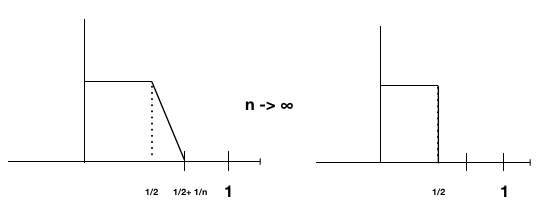
\includegraphics[width=0.5\linewidth]{Screen Shot 2024-01-21 at 10.59.57.png}
    \caption{Una función $C^0[0,1]$ }
    \label{fig:1}
\end{figure}

\underline{Ejemplos}
\begin{enumerate}
    \item $C^0( \Bar{\Omega} ) \text{ con } |f|_{0} = \underset{\Bar{\Omega}}{\max} |f(x)| $
    \item $C^1(\Bar{\Omega} ) \text{ con } |f|_{1} $
    \item $L^2(\Omega)$ por definición   $ = \{ f con  \{ f_n\}  \text{ continua, }  \iint |f_n -f_m|^2 < \infty  \text{ con } f_n \rightarrow f  \text{ y } \iint |f|^2<\infty  \} $
    \item $H^1(\Omega)$
\end{enumerate}

Sea $U\equiv \text{Vecindad de } f \in E  \Rightarrow \{ U \in E \} \supset  \{ g \text{  con  } || g - f || < \epsilon \}$,
definimos un punto de acumulación de $A\subset E$ ,  si $f\in E $ es punto de acumulación de $A$ si 
existe una sucesión $ \{ f_n \} \in A $ con  $f_n\rightarrow f$.

$\Bar{A} = \text{cerradura}  = A \cup \{ \text{puntos de acumulación} \} $


$A \text{ es \underline{ denso } en } E \text{ si } \Bar{A}  = E $


$Q$ es denso en $\mathbb{R}$


$\{ Polinomios\} $ denso en $L^2(\Omega)$


$\{\Bar{\Omega} \text{ compacto denso en } | |_0  \} \subset  C^0(\Omega)$ Stone-Weistrass

 
$E$ de Banach es \underline{separable} si existe un conjunto numerable denso en $E$


$C^0(\Bar{\Omega})$ es separable 


$L^2(\Omega)$ es separable 

Polinomios con coeficientes en $\mathbb{Q}+i\mathbb{Q}$ es separable

\section{Dependencia lineal}

Sea $E$ normado $f_1,..., f_n \in E$ son linealmente dependientes si existen $\lambda_1,...,\lambda_n$ escalares no todos cero
tales que


$\sum\limits_1^n \lambda_i f_i =0 \text{ en } C^0(\Bar{ \Omega}) : \sum\limits \lambda_i f_i(x) =0 \forall x\in  \Bar{ \Omega}$

$L^2(\Bar{\Omega} \Rightarrow \sum\limits \lambda_i f_i(x) = 0 $ \text{ a.e (almost everywhere) }

\begin{lemma}
Si $E$ tiene producto escalar, $f_1,...,f_n$ son linealmente independientes si y solo si
$D=$ matriz.  $D_{ij}= (f_i,f_j)$ es singular 
\end{lemma}

\begin{proof}
"$\Rightarrow$"  Si $\sum\limits_{j=1}^n \lambda_jf_j = 0 $   $\Rightarrow (f_i,\sum\limits_{j=1}^n \lambda_jf_j ) = \sum\limits_{j=1}^n \lambda_j (f_i, f_j ) =  \sum\limits_{j=1}^n  D_{ij} \lambda_j$
Es un sistema lineal de ecuaciones homogeneo, que para que tenga solución distinta de cero su determinante debe ser cero.
\end{proof}

\begin{ejemplo}
    \begin{enumerate}
        \item $L^2[0,1]$  $1,t,t^2,t^3,...,$ son linealmente independientes
        $(t^i, t^j)= \int_0^1 t^i t^j dt = \frac{1}{i+j+1}$

        \[
        D= \left( 
        \begin{array}{ccccc}
            1& \frac{1}{2}& \frac{1}{3}& \cdots& \frac{1}{n} \\
            \vdots & & & &\\
            \frac{1}{n} &&& & \frac{1}{2n+1}
        \end{array}
        \right)
        \]
    Se puede ver que su determinate no es cero    
    \item $L^2[0,\pi]$  $1,\cos x, \cos 2 x, ..., \cos n x$ son linealmente independientes. $D$ es diagonal,
    tambien $1,\sin x, \sin 2 x,..., \sin n x $ 
    \item $L^2 [0,2\pi]$  $1,\cos x, \sin x, \cos 2x, \sin 2x,..., \cos nx, \sin nx $ son linealmente independientes $D$ diagonal
    \item $L^2_{\mathbb{C}}[0,2 \pi]$   $e^{ijx}, j=-N,...,M$
    
    \end{enumerate}
    
\end{ejemplo}

\begin{definition}
$f \perp g  \Leftrightarrow (f,g) = 0$ 
\end{definition}

\begin{definition}
$\underset{f_i\neq 0}{\{f_1,...,f_n\}}\in \underset{(,)}{E}$ son ortogonales si $(f_i,f_j) = 0 \; i\neq j $ y son \underline{ortonormales} si $(f_i,f_j) = \delta_{ij}$ 
\end{definition}

\begin{theorem}
Sean $\phi_1,...,\phi_n,...$ ortonormales en $E$ con $(,)$
sea $U\in E$ y $ U_n = \sum\limits_1^n (U,\varphi_j) \varphi_j = \sum\limits_1^n \alpha_j \varphi_j$
$\alpha_j$ se llaman los coeficientes de Fourier de $U: L^2_{\mathbb{C}} [0,\pi ] , \phi $

Si $\varphi_j = \frac{ e^{ijx} } {\sqrt{2\pi}}$
\[
(\varphi_k,\varphi_j)= \int_0^{2\pi} \frac{e^{ikx}}{\sqrt{ 2\pi}} \frac{e^{-ijx}}{\sqrt{ 2\pi}} dx= \frac{1}{2\pi} \int_0^{2\pi} e^{i(k-j)}x dx = \delta_{ij}
\]

\[
\alpha_j=\frac{1}{\sqrt{2 \pi}} \int_0^{2\pi} U(x) e^{-ijx} dx
\]

$\Rightarrow$

\begin{enumerate}
    \item $\Vert U-U_n \Vert \leq \Vert U - \sum\limits_1^n \lambda_j \varphi_j \Vert \;\; \forall \;\; \lambda_1,\ldots, \lambda_n$ con igualdad solo si $\lambda_j= \alpha_j$



\item Desigualdad de Bessel  
\[
\sum_1^{n} |\alpha_j|^2 \leq \Vert U \Vert^2 
\]
y si $E$ es de Hilbert $\Rightarrow$  $\sum\limits_1^n \alpha_j \varphi_j$ converge en $E$ 

\item Si $\sum\limits_1^n \lambda_j^{(n)} \varphi_j  \overset{n\rightarrow \infty}{\longrightarrow }  U \Rightarrow  \lambda_j^{(n)}\overset{n\rightarrow \infty}{\longrightarrow }  \alpha_j , \sum\limits_1^n \alpha_j \varphi_j \rightarrow U  $

\[
\sum_1^{n} |\alpha_j|^2 =  \Vert U \Vert^2  \; \; \text{identidad de parseval}
\]
\end{enumerate}

\end{theorem}

\begin{proof}

\begin{figure}[H]
    \centering
    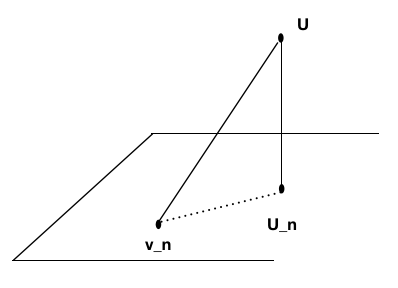
\includegraphics[width=0.5\linewidth]{Fig_2.png}
    \caption{Proyección ortogonal de U sobre $E_n= < \varphi_1, \ldots, \varphi_n >$ }
    \label{fig:2}
\end{figure}

    1)  sea $v_n = \sum\limits_1^n \lambda_j\varphi $ y $(\varphi_j,U) = \bar{\alpha}_j$
    entonces 
    
    \begin{align*}
    \vert U - v_n\Vert^2  &= ( U - \sum\limits_1^n \lambda_j\varphi_j , U - \sum\limits_1^n\lambda_j \varphi_j) \\    
    &= \Vert U \Vert^2 - \sum (\lambda_j \bar{\alpha}_j +\bar{\lambda}_j \alpha_j) +\sum|\lambda_j |^2\\
    &= \Vert U\Vert ^2  + (\sum (\lambda_j-\alpha_j) \varphi_j, \sum (\lambda_j-\alpha_j ) \varphi_j) - \sum |\alpha_j|^2
    \end{align*}

    tambien 
    \[
    \Vert U- U_n \Vert  \underset{\lambda_j = \alpha_j}{ =}  \Vert U\Vert^2 -\sum |\alpha_j|^2 
    \]
    \[
    \Vert U -v_n \Vert^2 \underset{\text{pitagoras}}{=} \Vert U - U_n\Vert^2 + \Vert U_n -v_n\Vert ^2  
    \]
    \[
    \Rightarrow \Vert U -U_n\Vert \leq \Vert U -v_n \Vert \text{con igualdad solo si  } v_n=U_n
    \]
    
\end{proof}

Lo volvemos a enunciar

\begin{theorem}
\label{Theorem:1}
Sea $H$ con  producto interno $(,)$, $\varphi_1,\varphi_2\ldots$  ortonormales  
\[
U\rightarrow U_n = \sum\limits_1^n (U,\varphi_j)\varphi_j
\]

\begin{enumerate}
    \item $\Vert U-U_n\Vert \leq \Vert U- v_n\Vert  \forall v_n = \sum\limits_1^n \lambda_j\varphi_j$
    \item $\sum\limits_1^n |(U,\varphi_j)|^2 \leq \Vert U\Vert ^2  \text{(Bessel)}$
    
    Si $H$ es de Hilbert $\Rightarrow \sum\limits_1^n (U,\varphi) \varphi_j $ converge a $v$
    \item si $v_n \rightarrow U  \Rightarrow \lambda_j^{(n)} \rightarrow (U,\varphi_j)$ , 
    
    $\sum\limits_1^n |(U,\varphi_j)|^2 = \Vert U \Vert^2$,
    
    $\sum\limits_{1}^{\infty} (U,\varphi_j) \varphi_j = U$
    
\end{enumerate}
\end{theorem}

\begin{definition}
\begin{enumerate}[label=\alph*]

\item) $\{f_1,f_2,\ldots   \}\in E$ es completo si todo $U\in E$ es aproximado por combinaciones finitas
$\Vert U-\sum\limits_1^n \lambda_j f_j \Vert \leq \epsilon$
\item) $E$ con $(,)$  y $\{ f_1,f_2,\ldots\}$ es cerrado si cuando $(U,f_j)=0 \forall i \Rightarrow U=0$ 
\end{enumerate}
\end{definition}

\begin{theorem}
    $H$ es de Hilbert cuando $\varphi_1,\varphi_2,\ldots$  son ortonormales 
    
    (1) $ \{ \varphi_1, \varphi_2,\ldots\}$ completa  $\Leftrightarrow (2) \{ \varphi_1,\varphi_2,\ldots \}$ cerrada    $\Leftrightarrow$(3) $H$  es separable  $\Leftrightarrow$ todo $U\in H $ se escribe como $U= \sum\limits_1^\infty (U_j,\varphi_j) \varphi_j$

    (4) $\{ \varphi_j \}$ son base de $H$ En general (si $\varphi_j$ no son $\perp$ ) completo $\Rightarrow$ cerrado
\end{theorem}

\begin{proof}
    (1) $\Rightarrow$ (4).  (3) del teorema anterior (\ref{Theorem:1}). (4) $\Rightarrow$ (1)  $ U= \sum\limits_1^\infty (U,\varphi_j)  \varphi_j =  \lim U_n   \underset{\lambda_j = (U,\varphi_j)}
    {U_n \rightarrow U }$

    (1) $\Rightarrow$ (2)  si $ (U,\varphi_j)=0 \forall j  \overset{(4)}{\Rightarrow} U=0$  
    
    (2) $\Rightarrow$ (1) Sea $w=U - \sum\limits_1^\infty (U,\varphi_j)\varphi_j$ $v de (2) anterior$
    $(w,\varphi_k)= (U,\varphi_k) -(U,\varphi_k) =0  \Rightarrow w= 0 \Rightarrow (4)\cong (1) $

    (1) $\Rightarrow$ (3) Dado $\epsilon \Rightarrow \Vert U - \sum\limits_1^n \lambda_j \varphi_j \Vert \leq \frac{\epsilon}{2} $

    $\sum\limits_1^n| \lambda_j - P_j| < \frac{\epsilon}{2}$ $P_j \in \mathbb{Q} + i \mathbb{Q} \Rightarrow \Vert U - \sum\limits_1^n P_j \varphi_j \Vert \leq \epsilon$

    (3) $\Rightarrow$ (4) Existe $\{ f_1,f_2,\ldots\}$ denso en $H$.

    Sea $\{g_1,g_2, \ldots\}\in \{ f_1,f_2,\ldots\}$ linealmente independientes

    $f_k = \sum\limits_1^k \lambda_j g_j$

    Aquí usamos la construcción de \underline{Gramm-Schmith}, sea $\varphi_1= \frac{g_1}{\Vert g_1\Vert}$

    $\tilde{\varphi}_2 = g_2 - (g_2,\varphi_1) \varphi_1 \perp \varphi_1 \;\; \tilde{\varphi}_2\neq 0$  

    $\varphi_2=\frac{\tilde{\varphi}_2}{\Vert \tilde{\varphi}_2\Vert}$

    $\tilde{\varphi}_3= g_3 -(g_3,\varphi_1) \varphi_1 - (g_3,\varphi_2)\varphi_2 \perp \varphi_1,\varphi_2 \neq 0$

    si $U\in H \Rightarrow \Vert U - f_n \Vert \leq \ep $  donde  $ \Vert U - f_n \Vert = \Vert U - \sum\limits_1^n \lambda_j g_j \Vert = \Vert U -\sum\limits_1^n \tilde{\lambda_j} \varphi_j \Vert$ 
\end{proof}

\begin{enumerate}
    
    \item $L^2_{\mathbb{C}} [ 0 , 2\pi] \;\;  \varphi_n=\frac{e^{inx}}{\sqrt{2\pi}} \;\; n=-\infty,\ldots,\infty$
    \item  $L^2_{\mathbb{R}} [ 0 , 2\pi] \;\;
 \varphi_n  = \left\{\begin{aligned}
       \frac{1}{ \sqrt{2\pi} }   &\;\;\;&  n= 0 \\
        \frac{1}{\sqrt{\pi}} \cos n x , \frac{1}{\sqrt{\pi}} \sin n x &\;\;\;&  n>0\\
       \end{aligned}
 \right. $
 \item $L^2[0,\pi]$
  $\varphi_n  = \left\{\begin{aligned}
       \frac{1}{ \sqrt{\pi} }   &\;\;\;&  n= 0 \\
        \frac{1}{\sqrt{\pi/2}} \cos n x &\;\;\;&  n>0\\
       \end{aligned}
 \right\}  \text{ó} \;\; \varphi_n \left\{ \frac{\sin nx}{\sqrt{\pi/2}} \right\}_{n>0} $
 en particular

 \[1=\sum\limits_0^\infty \left( 1,\frac{\sin n x}{ \sqrt{\pi/2}} \right) \frac{\sin nx }{\sqrt{\pi/2}} = \frac{4}{\pi} \sum_0^\infty \frac{\sin (2n+1)x}{2n+1}\]

  \text{porque}
  $\left( 1,\frac{\sin n x}{ \sqrt{\pi/2}} \right) = \int_0^\pi \frac{\sin n x}{ \sqrt{\pi/2}}  dx = \left.-\frac{1}{ \sqrt{\pi/2}} \frac{\cos nx}{n}\right|_0^\pi$

  \item $L^2 [a,b]$  $\frac{d^k}{dt^k} \left[ (t-a)^k (t-b)^k\right]$ polinomios de Laguerre 
  \item $L^2(\mathbb{R} )$ \text{Hermite} $\varphi_k =\frac{(-1)^k}{ 2^k k! \sqrt{2\pi}}  e^{\frac{t^2}{2} } \frac{d^k}{ dt^k} e^{-t^2}$   
  \item $L^2(\mathbb{R}^+ )$ Laguerre  $\varphi_k = \frac{e^{t/2}}{ k!} \frac{d^k }{dt^k} (t^k e^{-t})$
 \end{enumerate}


 \begin{definition}
\begin{enumerate}[label=\alph*]

\item) Complemento ortogonal y proyecciones. Sea $H$ de Hilbert, $M \subset H$ espacio lineal $\Rightarrow \bar{M}$ es lineal
y cerrado $\Rightarrow \bar{M} $ es de Hilbert.

\underline{Def:} $M^\perp = \{ U\in H \text{con} (U,v) = 0 \forall v\in M\}$
$M^\perp$ es lineal y cerrado, i.e.  $U_n\rightarrow U \text{y}$ donde cada $(U_n,v)=0 \forall v\in M$,
entonces
$|(U-U_n,v) |\leq \Vert U-U_n\Vert \Vert v\Vert \rightarrow 0$

\end{enumerate}
\end{definition}

\begin{propiedades}
\begin{enumerate}
    \item ) $M\subset N \Rightarrow N^\perp \subset M^\perp$  
    si $U\in N^\perp  \Leftrightarrow  (U,v) =0 \forall v\in N\supset M \Rightarrow U\in M^\perp $
    \item  $\bar{M}^\perp = M^\perp $   $M\subset \bar{M}  \overset{(1)}{\Rightarrow } \bar{M}^\perp \subset M^\perp $
    
    si $v\in M^\perp \Rightarrow (U,v)  = 0 \forall  v \in M$

    si $v\in \bar{M} \Rightarrow  v= lim v_n  \; \; v_n\in M$ 

    $(U, \underset{ \underset{v}{\downarrow}}{v_n})= 0  \Rightarrow (U,v)=0,  \Rightarrow U \in \bar{M}^\perp $

    \item Descomposición ortogonal. $M$ lineal, $U\in H \Rightarrow$ existe único $v\in \bar{M}$ con $U-v\in M $ y $\Vert U -v \Vert =\underset{z\in M}{inf} \Vert U-z \Vert \Rightarrow  U = \underset{\underset{M }{\rotin}}{v} + \underset{\underset{M^\perp }{\rotin}}{\underbrace{U -v}}$ 

    \[H= \bar{M} \oplus  M^{\perp}\]

    \begin{proof}
        Sea $d=\underset{z\in \bar{M}}{Inf}\Vert U-z\Vert$, sean $z_n\in \bar{M}$ con $\Vert U-z_n\Vert = d_n \rightarrow d$

        $\Vert z_n-z_m\Vert^2 = 2 \Vert U-z_n\Vert^2 + 2 \Vert U - z_m\Vert^2 -4 \Vert U-\frac{z_n + z_m}{2}\Vert^2$
        \text{Es la identidad del Rombo}

        $a,b\in H$ con $(,)$

        $\Vert a+b\Vert^2 + \Vert a - b \Vert^2 = 2\Vert a \Vert^2 + 2 \Vert b \Vert^2 $

        con $a= U-z_n$, $ b= U- z_m$, $\frac{z_n + z_m }{2} \in \bar{M} \Rightarrow \Vert U - \frac{z_n+z_m}{2} \Vert \geq d \;\; \text{cuando }  n,m \rightarrow \infty \Rightarrow \Vert z_n-z_m \Vert^2 \leq 2 d_n + 2 d_m - 4 d^2 \rightarrow 0  \Rightarrow \{z_n\} $ es de Cauchy $\overset{\bar{M}}{\rightarrow} v $ con $\Vert U-v \Vert = \lim\limits_{n\rightarrow \infty } d_n = d$

        \underline{v es único} si $\Vert U-v_1\Vert = \Vert U-v_2\Vert = d$
        y como
        $\Vert v_1-v_2 \Vert^2 = 2 \Vert U- v_1\Vert^2 + 2 \Vert U - v_2\Vert^2 -4\Vert U- \frac{v_1+v_2}{2}\Vert^2 \leq 2 d^2 + 2 d^2 -4d^2 =0 $

        $\Rightarrow v_1 = v_2$

        
        Ahora probar que $U-v\perp  M^\perp $. Sea $w\in \bar{M}$, $U-v -\epsilon w $ donde $v+\epsilon w \in \bar{M}$

        \[d^2 \leq \Vert U-v-\epsilon w\Vert^2 = \Vert U-v\Vert^2 +|\ep|^2 \Vert w\Vert - \bar{\ep} (U -v, w) -\ep (w,U-v) \]

        Sea $(U-v,w)= a e^{i\varphi}$  Sea $\ep= \rho e^{i\varphi} $ entonces la anterior desigualdad se convierte en
        
        \[ 0\leq \rho^2 \Vert w\Vert^2 -2 a \rho \;\; \forall \rho \]

        cambia designo para $\rho$ pequeño a menos que $a=0$

        \[\Rightarrow (U-v,w)=0\]

    \end{proof}
    
\end{enumerate}

\end{propiedades}

\begin{propiedades} $M\subset H$ $H$ de Hilbert  $M^\perp$ cerrado 
\begin{enumerate}
    \item $M\subset N \Rightarrow N^\perp \subset M^\perp$
    \item $\bar{M}^\perp = M^\perp$
    \item $\forall U \in H \Rightarrow \text{existe un único  } v \in \bar{M}$

    con $ U - v \in M^\perp \; \;  \Vert U-v\Vert = \underset{z\in \bar{M}}{inf} \Vert U-z\Vert$ Fig. (\ref{fig:3})
    entonces $u= \underset{\underset{\bar{M}}{\rotin}}{v} \oplus \underset{\underset{\bar{M}^\perp}{\rotin}}{u -v}$
    \begin{figure}[H]
        \centering
        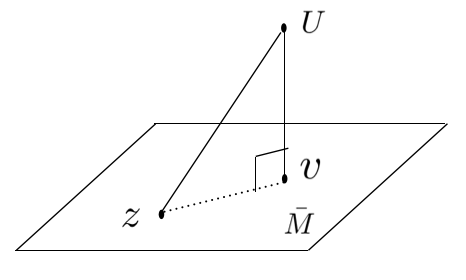
\includegraphics[width=0.5\linewidth]{Screen Shot 2024-02-10 at 18.39.45.png}
        \caption{Enter Caption}
        \label{fig:3}
    \end{figure}
    \item $(M^\perp ) ^\perp = \bar{M}$

    \begin{proof}
        $(M^\perp)^\perp = \{ U : (U,v) =0 \;\; \forall v \in M^\perp\}$ 
        si $U\in \bar{M} \Rightarrow u \perp v  \in  \bar{M}^\perp \Rightarrow \subset (M^\perp) $

        si la inclusión es estricta $\Rightarrow$ existe $U\in (M^\perp)^\perp $ y $U\notin \bar{M}$  $\Rightarrow \exists v \in \bar{M} $  tal que  
        $U-v \in M^\perp $, $\underset{\underset{\bar{M}}{\rotnotin}}{U} = v\notin \bar{M}$
    \end{proof}
    
\end{enumerate}
\end{propiedades}
    
\begin{ejemplo}
    $H=H^1[a,b] = \{ U(x) con \Vert U \Vert_1^2= \int_a^b U^2 + {U'}^2 < \infty \}$

    $= \{ U \text{limites en }  \Vert\;\; \Vert_1 \text{de sucesiones de Cauchy de funciones } C^1 \}$

    $\{ U_n \}\in C^1$  tales que $\Vert U_n - U_m\Vert_1 \leq \ep, \; \;\; n,m\geq N$ 
    
    si $x>y$  entonces $U_n(x)-U_n(x)\leq \int_y^x U_n'(x) d\tau $

    \[| U_n(x)-U_n(x) | \leq \int_y^x 1 |U_n'| d\tau \leq \left(  \int_x^y  d\tau \right)^{1/2}  \left( \int_x^y {U_n'}^2 d\tau \right)^{1/2} \]
    \[ \leq (x-y)^{1/2} \left(\int_a^b {U_n'}^2 d\tau \right)^{1/2} \leq |y-x|^{1/2} \Vert U_n \Vert_1\]

    Para $U_n-U_m \Rightarrow | U_n(x) - U_m(x) - ( U_n(y) -U_m(y) )| \leq |y-x|^{1/2}\Vert U_n-U_m \Vert$ 

    $\Rightarrow \{ U_n\}$ es de Cauchy en la norma $C^{0,1/2}$ 
    $=\{ U \text{Holder continua con exponente} 1/2 \}  $

    \[ |U(x)-U(y)|\leq K |x-y|^{1/2}\]

    \[\Vert U\Vert_{C^{0,1/2} } = max | U(x) | + \underset{x\neq y} { \max  } \frac{|U(x)-U(y)|}{|x-y|^{1/2}} \]

    
    \[\Rightarrow H^1[a,b] \subset C^{0,1/2}[a,b]\]
    
    $U(a)$ y $U(b)$ están definidos

    
    Sea  $ H_0^1[a,b] \equiv \{ U \in H^1 \text{ con } U(a)=U(b)= 0 \}$

    es un subespacio cerrado de $H^1$

    $M_0= \{ U \in C^1 \text{con} U(a)= U(b)= 0 \}$

    $M_0= H_0^1 \text{  si  } U\in {H_0^1}^\perp \Leftrightarrow (U,h)_1=0   \: \forall h \in H_0^1 $

    donde $(U,h)_1 = \int_a^b U h + U' h =0 \forall h \in C_0^\infty \subset H_0^1$

    $U$ es un punto crítico de $\int_a^b U^2 + {U'}^2 $  

    $\underset{euler}{\Rightarrow}$ $\frac{d}{dx} U'= U$   ($U$ es $C^2$)  entonces $U=Ae^{x} + B e^{-x}$

    $\Rightarrow \dim {H_0^1}^\perp = 2 $
    
    
\end{ejemplo}

\begin{ejemplo}
    Sea $ \Omega$ acotado en $\mathbb{R}^2$ decente $C^\infty$ (fluidos)  

    $M=\{ \nabla f= ( f_1.f_2) \text{  con  } f \in C^\infty (\bar{\Omega}) \} $

    $H = \widehat{M}^{\Vert \Vert_{L^2}} =  \{ (f_1,f_2)  \text{  y que existan  }  f_n C^\infty \text{  con  }  \nabla f_n \overset{L^2}{\rightarrow}(f_1,f_2)  \}$ es de Hilbert

    $M_0 =\{ \nabla f \in M \text{ con } f\in C_0^\infty   \} \;\; H_0= \bar{M_0}$
    
    $M_1= \{ \nabla f \in M \text{ con } \nabla^2 f = 0  \} \;\; H_1= \bar{M_1} $

    $(g_1,g_2) \in H_1 \Leftrightarrow \text{ existe } g_n  \text{ con }  \Delta g_n = 0 $

    $ \nabla g_n \overset{L^2}{\rightarrow} (g_1,g_2) $

    $ H = H_0 \oplus  H_1$

    \begin{proof}

    \begin{enumerate}
        \item \[ M_0 \perp M_1 : \iint \nabla f \cdot \nabla g = - \iint_\Omega  f \underset{  \underset{0}{\parallel}  }{\Delta g}  + \int_{\partial \Omega} \underset{  \underset{0}{\parallel}  }{f} \frac{\partial g}{ \partial n} = 0\]

        Si $\bar{f} = (f_1,f_2) \in H_0 $
    
        Si $\bar{g} = (g_1,g_2) \in H_1 $

        $(\bar{f},\bar{g}) = ( \bar{f} - \nabla f_n ,\bar{g} ) + \overset{0}{\overset{||}{\overbrace{ ( \nabla f_n, \nabla g_n ) } } } + (\nabla f_n, \bar{g} - \nabla g_n  )$ 

        $\leq \underset{ \underset{0}{\downarrow}}{ \underbrace{ \Vert \bar{f} -\nabla f_n \Vert } }  \Vert g\Vert + 
        \underset{\underset{\Vert \bar{f} \Vert}{\downarrow}}{\Vert \nabla f_n \Vert} \underset{\underset{0}{\downarrow}}{\underbrace{\Vert \bar{g}- \nabla g_n\Vert} } $  Prueba que el producto interno es continuo

        \item $H_0 \perp H_1 $ 
        \item $H_1^\perp = H_0$

         si $\bar{f}= (f_1,f_2)$ es $\perp$ a $H_1$ 
         
         $(\bar{f},\bar{g}) =0 \; \forall \bar{g} \in H_1 \supset M_1$

         $(\bar{f},\nabla g) = 0 \; \forall \nabla g \in M_1$

         Sean $f_n\in M$

         con $\nabla f_n \rightarrow \bar{f}$

         $(\nabla f_n , \nabla g) = \iint_\Omega \nabla f_n\cdot \nabla g = - \iint_\Omega f_n \underset{\underset{0}{||}}{\Delta g} + \int_{\partial \Omega} f_n \frac{\partial g}{\partial n} $


         $(\nabla f_n , \nabla g) \rightarrow (\bar{f},\nabla g)=0$

         $\int_{\partial \Omega} f_n \frac{\partial g}{\partial n}  \overset{n\rightarrow \infty}{\rightarrow}0 \;\; \forall \nabla g \in M_1$

         $f_n$ es tal que $\nabla f_n \in L^2 \Rightarrow f_n \in H^1 (\Omega) $

        $\Rightarrow f_n|_{\partial \Omega } \in L^2 (\partial \Omega) $ (teorema de traza)

        $\Rightarrow f_n |_{\partial \Omega} \rightarrow f$  en $L^2(\partial \Omega) $ con $\iint_\Omega f \frac{\partial g}{ \partial n} = 0 \; \forall g \in M_1$

        Sea $h\in C^\infty(\partial \Omega) $ con $\int _{\partial\Omega } h= 0$

        $ \left\{\begin{aligned}
        \Delta g = 0 \text{ en } \Omega \\
        \frac{\partial g}{\partial n }= h \text{ en } \partial \Omega \\
       \end{aligned} \text{ tiene solución única + constante (Neuman }
        \right. $

        si $\int_{\partial \Omega } h  = 0  \left\{   \begin{aligned}
            h \perp \text{const}\\
            h \in L^2(\partial\Omega)
        \end{aligned}
        \right.
        $
        
        $\int_{\partial \Omega} f h = 0 \Rightarrow f\perp L^2(\partial \Omega) $

        $\Rightarrow f_n |_{\partial \Omega} \rightarrow f \text{ en } L^2(\partial \Omega) $

        
     \end{enumerate}
        


        
        
        
    
    \end{proof}


    
\end{ejemplo}

\section{Operadores y funcionales}

\begin{ejemplo}
    Temperatura $T(x,y,z)$  en $\Omega$ equilibrio térmico. 
    
    Si no hay fuentes entonces $\nabla^2 T= 0$ si $T|_{\partial \Omega = f }$ dada
    
    Entonces $T= K_1 f$ donde $K_1$ es un operador lineal. 
    
    ¿Que propiedades tiene $K_1$, o que espacios, es un operador continuo? 

    Si en la frontera $\frac{\partial T}{ \partial n} =  g$  flujo de calor dado
    
    entonces $T=K_2 g $  $K_2$ operador lineal. 
    
    Si $\int_{\partial \Omega} g = 0$ y
    $T$ perpendicular a las constantes es el problema de Neuman. 

    Si el ambiente está a la temperatura $T_0$ entonces la ley de enfriamento es

    $\frac{\partial T }{ \partial n } + k (T-T_0) = h(x,y,z) $ Es el problema de Robin

    entonces $T= k_3 h$

    Si hay fuentes $\Delta T = k(x,y,z)$  

    $T= \underset{\underset{\text{con datos homogeneos }}{\downarrow}}{K} k + K_i f$
\end{ejemplo}


\begin{definition}
 Sea \underline{Operador}  $A: H \rightarrow K$  espacios lineales

 $D(A)= \text{ dominio de } A = \{ U\in H \text{ tal que } AU \text{ tenga sentido }$ \}

 $R(A) = \text{ Rango de } A = \{ v \in  K \;\; v= A v\}$ 

 $Ker A= \{  U \text{ con } Au=0\}$

 $A$ es un funcional si $K= \mathbb{R} \text{ ó } \mathbb{C}$  
\end{definition}

\begin{ejemplo}
    \begin{enumerate}
        \item $A=\Delta\;\;\;$ con $H= C^2(\bar{\Omega} )$ y $K= C^0(\bar{\Omega})$ y $D(A)=H$  
        \item $A=\Delta \text{  con } H= L^2 (\Omega)  = K \text{ y }  D(A)\subset H^2(\Omega) $
        \item $A=\Delta \text{ con  } H= C^2(\Omega) \cap \{ U=0 \text{ en } \partial\Omega\}$
        \item $H= L^2 \text{ con } A(U) = \iint_{\Omega} |U|^2 dx \in \mathbb{R} \text{ no es lineal} $ 
        \item $A U(x) = \iint_\Omega k(x,y) U(y) dy $,  $k(x,y)$ es el nucleo, $x\in \Omega\subset \mathbb{R}^3$

    \[
    k(x,y)  = \left\{\begin{aligned}
        \frac{1}{|x-y|^{n-2}}  & \text{ si } n> 2 \\
         \log(x-y ) & \text{ si } n = 2,
       \end{aligned}
    \right.
    \]

    es un operador lineal 

    $D(A)$  lineal si
    
    $A(U+v) = A U  + A v$
    
    $A(\lambda U ) = \lambda A U $
    
    
     \end{enumerate}
\end{ejemplo}

\underline{Inverso}: $A: H \rightarrow K$ si  $A$ 1-1, sobre entonces $D(A)=H$ 

$A^{-1}:K\rightarrow H$


si los espacios tienen norma

$A:H \rightarrow K$ lineal, $A$ es acotado si existe $M$ tal que $\Vert AU\Vert_K \leq M\Vert U\Vert_H$

$A$ lineal $\Rightarrow A $ es 1-1 $\Rightarrow Ker A= 0$ 

$Ax = Ay \Leftrightarrow A(x-y) =0 \Leftrightarrow x=y $

\underline{Norma de A} 

\[
\begin{array}{ll}
\Vert A\Vert      &  = Inf\; M= \underset{U\neq 0}{sup} \frac{\Vert A U\Vert_{K}}{\Vert U\Vert_H} \\
     & = \underset{0<\Vert U\Vert_H\leq1 }{ sup} \frac{\Vert A U\Vert_{K}}{\Vert U\Vert_H} \\
     & = \underset{\Vert U\Vert_H = 1 }{ sup} \Vert A U\Vert_K
\end{array}
\]

\begin{proposition}
    $A$ lineal, $A$ acotado $\Leftrightarrow $ $A$ es continua en $0$ $\Leftrightarrow$ $A$ es continua.
    
\end{proposition}
\begin{proof}
    $A: H\rightarrow K$ normados, $A$ lineal acotado 
    \[ \Vert A\Vert = min \; \text{cotas sup} \underset{x\neq0}{=} \frac{sup \Vert Ax\Vert}{\Vert x\Vert}\]
    entonces
    \[
    \Vert A x\Vert \leq \Vert A \Vert \Vert x \Vert
    \]
\end{proof}

\begin{proposition}
    (1) $A$ acotado $\Leftrightarrow$ (2) $A$ es continuo en $0$ $\Leftrightarrow$ (3) $A$ es continuo
\end{proposition}

\begin{proof}
    (1) $\Rightarrow$ (3) 

    $\Vert Ax - Ay \Vert = \Vert A(x-y)\Vert\leq \Vert A \Vert \Vert x-y \Vert$ es Lipshitz continuas

    (3) $\Rightarrow$ (2), (2) $\Rightarrow$ (1)

    $A$ continua en $0$ $\Leftrightarrow$ $\Vert Ax -\underset{\underset{0}{||}}{A0}\Vert \leq \epsilon $ si $\Vert x-0\Vert \leq \eta$

    sea $g=D(A)$ , $g\neq 0$, Sea $x=\eta \frac{y}{\Vert y\Vert}$ $\Vert x \Vert = \eta$

    \[\Vert Ay \Vert = \Vert Ax \Vert \frac{\Vert y \Vert}{\eta} \leq \frac{\epsilon}{\eta} \Vert y\Vert\]
    \[\Rightarrow \Vert A \Vert \leq \frac{\epsilon}{\eta}\]
    Nota: $\Vert AB\Vert \leq \Vert A\Vert \Vert B\Vert$
\end{proof}

\begin{ejemplo}
    Operador integral  $\Omega \subset \mathbb{R}^n $
    \[
    (KU)(x)=\iint_\Omega k(x,y) U(y) dy   
    \]
    es lineal $U\in L^2 (\Omega) $

    \begin{align*}
    \Vert KU \Vert ^2 & = \iint_\Omega (kU)^2 dx = \iint_\Omega  \left( \iint_\Omega k(x,y) U(y) dy \right)^2 dx \\
    &\underset{Cauchy-Shwarz}{\leq} \iint_\Omega \left( \iint_\Omega k^2 dy \iint_\Omega U^2(y) dy \right)dx \\
    & = \iint_\Omega \iint_\Omega k^2(x,y) dx dy \Vert U \Vert^2
    \end{align*}

    \[
    \text{Si   }  M^2 = \iint_\Omega \iint_\Omega k^2 dx dy \leq \infty
    \]

    \[
    \Rightarrow K: L^2 \rightarrow L^2 \text{   acotado}
    \]
    
    si $\Vert K \Vert \leq M $  se dice que $K$ es un operador de Hilbert-Schmidt    
\end{ejemplo}

\begin{ejemplo}
    $A U = U'$  donde $U \in L^2[0,1] $, $D(A)$ no es todo $C^0$ 
    \[
    U_n(x)= \sin n \pi x
    \]
    \[
    \Vert U_n\Vert_{L^2} = \left(  \int_0^1 \sin^2 n\pi x dx \right)^{1/2}= \frac{1}{\sqrt{2}}
    \]

    \[
    \Vert Au \Vert_{L^2} =\Vert U'\Vert = \left( \int_0^1 (n\pi)^2 \cos^2 n\pi x dx \right)^{1/2} = \frac{n\pi}{\sqrt{2}}
    \]

    $U_n$ son acotados pero $AU_n$ no, $A$ no es continua

    $D(A)\subset L^2 \rightarrow L^2$

\end{ejemplo}

\section{Proyección ortogonal}

\begin{figure}[H]
    \centering
    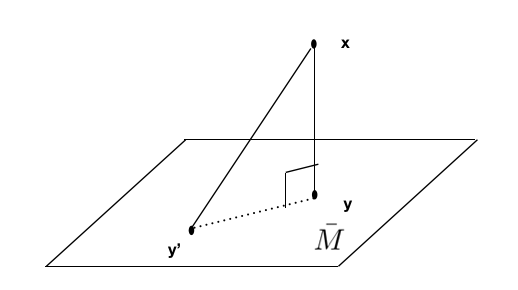
\includegraphics[width=0.5\linewidth]{Screen Shot 2024-03-03 at 06.55.16.png}
    \caption{}
    \label{fig:4}
\end{figure}

$H$ de  Hilbert, $M= \bar{M}\subset H$ , $x\in H \Leftrightarrow x= y + z$ donde $y\in M$, $z\in M^{\perp}$

Sea $Px = y $ es lineal

$x_1= y_1+ z_1$
$x_2 = y_2 + z_2 $

\[ 
x_1+x_2 = \underset{\underset{M}{\rotin}}{(y_1+y_2)} +\underset{\underset{M^{\perp}}{\rotin}}{(z_1+z_2)} 
\]

Por la unicidad de la proyección $P(x_1+x_2) = y_1+y_2= Px_1+Px_2$

$P^2x =P y = y = Px \Rightarrow P^2 = P$

$\Vert Px\Vert^2 = \Vert y\Vert^2 -\Vert x\Vert^2-\Vert z\Vert^2 \leq \Vert x\Vert^2$

$\Vert Px \Vert \leq \Vert x\Vert \leq 1$ para $y\in M \Rightarrow Py=y$


\underline{Nota:} Si $A: D(A)\subset H \rightarrow K $ $K$ de Banach lineal y continuo

$\Rightarrow$ uno puede extender $A$ a $\tilde{A}: H\rightarrow K $  

$\Vert\tilde{A}\Vert =\Vert A\Vert $ porque si $x\in \overline{D(A)} $  $x_n\in D(A) $ con $x_n \overset{H}{\rightarrow} x $

que puedo decir $\Vert A x_n - A x_m\Vert \leq \Vert A \Vert \Vert x_n -x_m$ 

$\{A x_n\}$ es de Cauchy en $K$ completo 

$ \Rightarrow Ax_n\rightarrow y $ independiente de $\{ x_n\rightarrow x\}$

Definimos $\tilde{ A x} =y$

\begin{align*}
 \Vert A x_n \Vert & \leq \Vert A \Vert \Vert x_n \Vert \\
 \downarrow &  \\
 \Vert A x \Vert &\leq \Vert A \Vert \Vert x \Vert \Rightarrow \Vert \tilde{A} \Vert = \Vert A \Vert
\end{align*}

$\overline{D(A)}$ cerrado en $H$ sobre $D(A)^\perp$ se define $\tilde{A}x =0$

$\Rightarrow \Vert \tilde{A} \Vert =\Vert A\Vert $


\section{Teorema de Representación de Riez}
 
Sea $L: H \rightarrow \mathbb{C} $ ó $\mathbb{R}$ un funcional lineal continuo

$\Rightarrow \exists  $ un único $l\in H$ talque $Lx=(x,l)$  y $\Vert L\Vert =\Vert l \Vert$

\begin{ejemplo}
    $H= H^1(0,1)$  $ LU = \int_0^1 f(x) U(x) dx =(f,U)_{L^2}$

    $L:H^1 \rightarrow \mathbb{R} $ lineal

    $|LU |\leq \Vert f\Vert_{L^2} \Vert U \Vert_{L^2} \leq \Vert f\Vert_{L^2} \Vert U \Vert_{H^1} $

    $\Rightarrow$ existe $l$ único con $LU= (l,u)_{H^1} = \int_0^1 l U +l' U' $
\end{ejemplo}

\begin{proof}
    Sea $M= Ker L \{ x | Lx =0 \}$

    \begin{enumerate}
        \item $M= \bar{M} $  cerrado  $\underset{\underset{x}{\downarrow}}{x_n}\in M$ por continuidad de $L$

        \item $M^\perp $ si $L\neq 0 $ existe $y_0$ con $L y_0 \neq 0$ 
        
        sea $y \in M^\perp \Rightarrow $  existe $\alpha = \frac{-Ly}{L y_0}$

        talque $L(\alpha y_0 +y ) = 0$ 

        $ \therefore  \alpha y_0 +y \in M $

        $\Rightarrow \dim M^\perp = 1$

        \item Si $x\in H \Rightarrow x= \beta y_0 + z $, $z\in M$

        $\beta = \frac{(x,y_0)}{\Vert y_0 \Vert^2}$

        $Lx = \beta L y_0 =( x,\frac{y_0 L y_0 }{\Vert y_0 \Vert^2}) = (x,l)$

        \item $l$ es única 

        si $Lx = ( x,l_1) = (x_1,l_2) $

        $\Rightarrow (x,l_1-l_2) =0  \forall x\in H \Rightarrow l_1=l2$

        \item $|Lx| =| (x,l) |\leq \Vert l\Vert \Vert x\Vert \Rightarrow \Vert L\Vert \leq \Vert l \Vert$

        $L l = \Vert l\Vert^2$
        
        $L l \leq \Vert L\Vert \Vert l \Vert$

        $ \Vert l\Vert \leq \Vert L \Vert$

        $\Rightarrow \Vert L \Vert = \Vert l \Vert$

        me puedo olvidar del espacio dual, el espacio dual de $H$ es $H$
        

        
    \end{enumerate}
\end{proof}

\section{Operadores simétricos, positivos}

Sea $A: D(A) \subset H \rightarrow H$ lineal  

\begin{definition}
    $A$ es \underline{simétrico} sí $D(A)$ es denso en $H$ 
    $\forall U,v \in D(A) : (U, Av)=(AU, v) $
\end{definition} 

\begin{ejemplo}
    $Au = -U''$ $D(A)\subset C^\infty$ $U\in L^2 [a,b] $

    \[
    (AU,v)= \int_a^b -U'' v dx = \int_a^b U'v' dx - U'v|_a^b
    \]
    \[
    =\int_a^b U v'' dx + (Uv' - U'v)|_a^b = (U,Av) + (U v'-U'v)|_a^b
    \]

es simétrico $\Leftrightarrow  (U v'-U'v)|_a^b=0 \forall U,v \in D(A)$ 

por ejemplo: condiciones de frontera separadas

\begin{align*}
  \alpha U(a) + \beta U'(b) = 0\\
  \gamma U(a) + \delta U'(b) = 0\\
\end{align*}

    
\end{ejemplo}

\begin{ejemplo}
    $AU= -\Delta U$ $U(x)$  $x\in \Omega \subset \mathbb{R}^n$  $U|_{\partial \Omega =0}$

    $H=L^2(\Omega)$ $D(A) \supset C_0^{\infty}$
    \[
    (U,Av)= \iint_\Omega -U \Delta v = \int_\Omega \nabla U\cdot \nabla v - \int _{\partial \Omega} \underset{\underset{0}{||}}{U} \frac{\partial v}{\partial n}  = (A U,v)
    \]
    
\end{ejemplo}



\section{Tarea}
\begin{enumerate}
    \item Probar que 
    \[
    (AU , v) = \frac{1}{4} \left[ (A(U+v) ,U+v) - (A(U-v),U-v) + \right.\]
    \[
    \left. i (A(U+iv),u+iv) - i (A(U-iv),U-iv) \right]
    \]
    \item 
    Probar que si $(AU,U) \in \mathbb{R} \forall U \Rightarrow A $ es simétrica
    (Usar ley desigualdad del rombo)
    \item Si $H$ es real, probar que $(AU, U)\geq 0$ $\nRightarrow $ que $A$ sea simétrica (Encontrar un ejemplo en $\mathbb{R}^2$) 
\end{enumerate}

\begin{ejemplo}
    Sea $AU=-\Delta U$ con $D(A) = C^2 (\bar{\Omega}) \cap \{ U|_{\partial \Omega} =0\}$ denso en $L^2(\Omega)$

    Entonces 

    \[
    (AU,U)= \iint_\Omega -\Delta U U = \iint_\Omega |\nabla U| ^2 > 0 
    \]
    
 excepto si $ \nabla U= 0$ $\Rightarrow  U\equiv 0 $

 $\Rightarrow -\Delta $ es definido positivo y es un poco más, es \underline{fuertemente positivo}
 
 \end{ejemplo}
\section{Desigualdad de Poincare}

Si $U \in H_0^1(\Omega) \Rightarrow $ existe $c$ tal que 

\[
\iint U^2 \leq c \iint_\Omega |\nabla U |^2 
\]

 \[
 (AU,U)= \iint _\Omega |\nabla U|^2 \geq \frac{1}{2} \iint_\Omega |\nabla U|^2 +\frac{1}{2c} \iint_\Omega U^2
 \]

 \[
 \geq \min \left( \frac{1}{2},\frac{1}{2c} \right) \Vert U \Vert_1^2
 \]

\section{Poincaré}

Sea $U\in H_0^1(\Omega)$

\[
\Rightarrow   \iint_\Omega U^2 \leq c \iint_\Omega |\nabla U | ^2 \]

\begin{proof}
     Sea $U\in C_0^\infty(\Omega) $ 
     \begin{figure}[H]
         \centering
         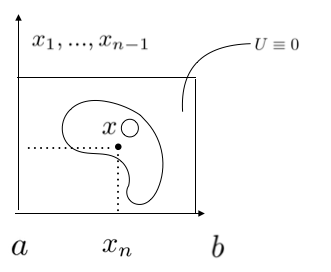
\includegraphics[width=0.5\linewidth]{Screen Shot 2024-03-06 at 21.12.47.png}
         \caption{}
         \label{fig:enter-label}
     \end{figure}
     \[U(x)= \int_a^{x_n} U_{x_n} ( x_1,...,x_{n-1} ,\xi )d\xi\]
     \[
     U(x)^2= \left(  \int_a^{x_n} 1 |U_{x_n}| d\xi \right)^2\leq \int_a^{x_n} 1 d\xi \int_a^{x_n} U_{x_n}^2 d\xi\leq (b-a) \int_a^b U_{x_n}^2 d\xi 
     \]
     \[
     \iint_\Omega U(x)^2 dx= \iint_{\square} U^2 dx \leq (b-a) \iint_{\square} \int_a^b  U_{x_n}^2 d\xi d x_1...d x_{n-1} dx_n
     \]
     \[
     =(b-a)^2 \iint U_{x_n}^2 dx_1 ... dx_{n-1} d\xi = (b-a)^2 \iint_\Omega U_{x_n}^2 dx 
     \]
     \[
     \leq (b-a)^2 \iint_\Omega |\nabla U|^2 dx
     \]
     
\end{proof}

$\Rightarrow $ Desigualdad es válida para $U\in C_0^\infty(\Omega)$ 

$C_0^\infty(\Omega)$ es denso en $H_0^1= (U_n\in C^1 , U_n|_{\partial \Omega} =0 , U_n \overset{H^1}{\rightarrow} U  )$ 

Sea $\rho : \mathbb{R}^n \rightarrow \mathbb{R}^+$,  $C^\infty$, $\rho(z) \equiv 0$ si $|z| \geq 1$

Sea $U\in L^2(\Omega)$ extendiendo $U\equiv 0$ fuera de $\Omega$ y tal que

\[\iint_{\mathbb{R}^n} \rho(z) dz= 1\]

Sea

\[
(J_\epsilon U )(x) = \frac{1}{\epsilon^n} \iint_{\mathbb{R}^n} \rho(x-y) U(y) dy
\]

donde $\rho(x-y)=0$ si $|x-y|\geq \epsilon$ 

 $\Rightarrow$  $J_\epsilon U $ es $C^\infty$ 

 si hacemos $z=\frac{y-x}{\ep}$ y $dz= \frac{1}{\ep^n} dy$ 
 \[
 J_\ep U(x) = \iint_{\mathbb{R}^n} \rho(z) U( x+\ep z) dz\]

Es el promedio de $U$ sobre una bola de centro $x$ y radio $\ep$. 

$J_\ep$ es un operador lineal sobre $L^2$

Si $U\in C(\Omega)$ entonces

\[
J_\ep U(x)-U(x) = \iint_{\mathbb{R}^n }\rho(z) \left(U(x+\ep z) -U(x)  \right) dz
\]

\[
\left| J_\ep U(x)-U(x) \right| \leq \iint_{\mathbb{R}^n }\rho(z) \left|U(x+\ep z) -U(x)  \right| dz
\]


$\left|U(x+\ep z) -U(x)  \right| \leq h$ si $\ep$ pequeño

$\Rightarrow$ $J_\ep U \overset{\ep\rightarrow 0}{\rightarrow} U $ en compactos de $\Omega$ .

$U \in C(\Omega) , U|_{ \partial \Omega} =0 \Rightarrow J_\ep U \overset{\text{uniforme}}{\underset{\ep \rightarrow 0}{\rightarrow}} U $ en $C(\bar{\Omega})$


Si $U$ es $C^1$ $\Rightarrow$  $J_\ep U \overset{\ep\rightarrow 0}{ \rightarrow} U $  en $C^1$ (compacto $\Omega$)

\[
\iint_\Omega ( J_\ep U - J_\ep v )^2 dx =\iint_\Omega \left( \iint_{\mathbb{R}^n} \rho (z) ( U(x+\ep z)) -v(x+\ep z) dz\right)^2 dx
\]

\[
=\iint_\Omega \underset{\underset{1}{||}}{ \underbrace{\iint_{\mathbb{R}^n} \rho (z) dz}}  \iint_{\mathbb{R}^n} \rho (z) ( U(x+\ep z)) -v(x+\ep z) )^2 dz dx
\] 

\[
\underset{\text{Fubbini}}{=} \iint_{\mathbb{R}^n} \rho (z) \left[  \iint_\Omega \left( U(x+\ep z) -v(x+\ep z) \right)^2 dx \right] dz 
\]

\[
=\iint_{\mathbb{R}^n} \rho(z) \underset{ \Vert U-v\Vert_{L^2}}{ \underbrace{ \iint_{\mathbb{R}^n} \left( U(w) -v(w)  \right)^2 dw  } } dz 
\]

$\Rightarrow \Vert J_\ep U -U\Vert_{L^2} \leq \Vert U-v\Vert $ en $L^2(\Omega) $  $J_\ep \leq 1$.

Sea $U \in H_0^1 (\Omega) \Leftrightarrow \exists U_n \in C^1$, $U_n|_{\partial \Omega} =0 $ y $U_n\underset{H^1}{\rightarrow}U$ 

\[
\Vert J_\ep U- U\Vert_{L^2} \leq \Vert J_\ep U -J_\ep U_n\Vert + \Vert J_\ep U_n -U_n\Vert + \Vert U_n-U\Vert
\]

\[
\leq 2 \underset{{\underset{0} {\downarrow} n\rightarrow \infty}}{\Vert U_n -U\Vert } + \Vert J_\ep U_n-U_n\Vert
\]

Ahora yo se que 

\[
\iint_\Omega \underset{\leq \eta' \text{ si } \ep< \ep_0 }{\underbrace {\left( J_\ep U_n -U_n\right)^2} }  dx \leq \eta' (vol \Omega )\leq \frac{\eta}{2}
\]

Por lo tanto

\[
\Vert J_\ep U - U \Vert_{L^2} \leq \eta
\]

Sea $U\in L^2 \Rightarrow \underset{\underset{C^\infty}{\rotin}}{J_\ep U} \underset{L^2}{\overset{\ep \rightarrow 0}{\rightarrow }}  U$ $\rightarrow$ $C^\infty (\Omega) $ es denso en $H^m(\Omega) = \widehat{C^m(\bar{\Omega})} ^{\Vert\;\Vert_m}$

\[
H_0^m(\Omega) = \widehat{C_0^m(\bar{\Omega})} ^{\Vert\;\Vert_m}
\]

donde

\[
\Vert U\Vert_m^2 = \sum\limits_{\alpha_1+...+\alpha_n = \alpha \leq m} \iint_\Omega \left( \frac{D^\alpha U }{D^{\alpha_1}_{x_1} \cdots D^{\alpha_1}_{x_n}  } \right)^2 dx
\]

Para $U\in C_0^\infty $

\[
\iint_\Omega U^2 \leq c\iint_\Omega |\nabla U\Vert^2
\]

Si $U\in H_0^1$ $U_n\in C_0^\infty \overset{H_1}{\rightarrow} U$

\[
\left( \iint_\Omega U^2 \right)^{1/2}= \Vert U\Vert \leq \Vert U -U_n\Vert + \Vert U_n\Vert
\]

\[
\left( \iint_\Omega |\nabla U|^2 \right)^{1/2}= \Vert U\Vert \leq \Vert  \nabla (U -U_n) \Vert + \Vert \nabla U_n\Vert
\]

\[
\Vert U \Vert \leq \Vert U -U_n \Vert + c\Vert \nabla U_n \Vert \leq \Vert U-U_n\Vert + c ( \Vert \nabla U \Vert + \Vert \nabla ( U-U_n)  \Vert )
\]

\[
\leq c \Vert \nabla U \Vert + (1+c)\Vert U- U_n\Vert_1 \forall n
\]

\[
n\rightarrow\infty \Rightarrow \Vert U \Vert \leq c \Vert\nabla U \Vert
\]

\chapter{MÉTODOS VARIACIONALES}

\begin{ejemplo}
    Ejemplos y resultados fundamentales

    \begin{enumerate}
        \item $U_{tt} -\Delta U=0$ con transformada de Laplace en $t$, $\hat{U}$
        \[ -k^2 \hat{U}^2 -\Delta \hat{U}=0\]
        $U|{\partial \Omega}  $ dado 

     \item   \underline{Estudiar}  $-\Delta U + q(x) U = f_1 $  en $\Omega$ con $U|_{\partial \Omega =g_1} $ Dirichlet  ó 

  $-\Delta U + q(x) U = f_2 $ con $\frac{\partial U}{\partial n}|_{\partial \Omega =g_2} $ Neuman
   \item $-\Delta U + q(x) U = f_3 $ con $U+h\frac{\partial U}{\partial n}|_{\partial \Omega =g_3} $ Robin     
    \end{enumerate}
\end{ejemplo}

Supongamos que existe $U_0\in C^2 (\bar{\Omega})$ tal que $\frac{\partial U_0 }{ \partial n}|_{\partial \Omega} =g_2 $ ó 
$\frac{\partial U_0 }{ \partial n} + h U_0|_{\partial \Omega}  =g_3 $

$\Rightarrow$ Sea $U = U_0 +W $, $-\Delta W +qW= f+\Delta U_0 -q U_0 \equiv \tilde{f} $ con $W|_{\partial \Omega} =0 $ ó $\frac{\partial W}{\partial n}|_{\partial \Omega} =0 $  

Por lo tanto podemos tomar datos de la frontera igual a cero 

Sea 
\[
E_i = \left\{ \begin{array}{llr}
     U\in C^2 (\bar{}\Omega), & U|_{\partial \Omega} = 0 & i=1  \\
     &  \frac{\partial U}{\partial \Omega}|_{\partial \Omega} = 0 & i=2 \\
     & \frac{\partial U}{\partial \Omega} + hU |_{\partial \Omega} = 0 & i=3 \\
\end{array} 
\right\}
\]

Es lineal

$A_i = -\Delta +q $ lineal sobre $E_i$

yo puedo tomar

\[
\iint_{\Omega} (A_i U) v dx = (A_i,v)  \]

 donde $U,v\in E_i$ 
\[
= \iint_{\Omega} \Delta U  v + q U v 
\]
\[
= \iint_{\Omega} \nabla U \cdot \nabla v + q Uv - \int_{\partial \Omega} v \frac{\partial v}{ \partial n}
\] 

Es simétrico si $\int_{\partial \Omega} v\frac{\partial U}{\partial n} = \int_{\partial \Omega} U \frac{\partial v }{\partial n} \forall \; U,v \in E_i$

en los tres epacios es simétrico 

\[
=\iint_{\Omega} \nabla U \cdot \nabla v + q U v + \int_{\partial \Omega} h U v 
\]

$h\equiv 0$, si $i=1,2$

es simétrico

$=(U,A_iv)$

\[
(A_i U , U) = \iint_\Omega |\nabla U |^2 + q U^2 + \int_{\partial \Omega} h U^2 \geq 0 \text{  si  } q\geq 0, h\geq 0
\]

Caso 1 $U=0$ si $i=1$

Caso 2 $U=cte$ si $i=2$

$\Rightarrow U=0$ si $\iint_\Omega q \geq 0 $  si $\{ x \text{con} q(x) >0 \text{ tiene medida >0 } \}$


Caso 3 $U=0$ para $i=3$ si $q>0$ en un conjunto de medida $>0$ ó $h>0$ en un conjunto de medida $>0$

Resolver $A_i U= f $  para $U\in E_i$

\begin{theorem}
    Sea $A$ con $D(A)$ denso en $H$ (Hilbert) real, $A$ simétrico $\geq 0$ 
    $\Rightarrow$  
    \begin{enumerate}
        \item $A>0 \Rightarrow$ si hay solución $(A U =f, U \in D(A) )\Rightarrow $ es única 
        \item $U$ solución $\Leftrightarrow I(U) = (AU,U) -2(f,U) $ es un mínimo en $U_0$ como funcional sobre $D(A)$
        es el principio de Dirichlet
    \end{enumerate}
\end{theorem}

\begin{proof}
    \begin{enumerate}[label=\alph*]
        \item) Si $AU=f$, $Av=f$

        
        $A(U-v) =0 , 0= (A(U-v),U-v)>0$ si $U\neq v$
        
        $\Rightarrow U=v$

        \item $\Rightarrow )$ $U= U_0 +h$ $U, U_0\in D(A)\Rightarrow h\in D(A)$ 

        \[
        I(U_0 +h) = ( A(U_0+h) ,U_0+h) -2 (f,U_0 +h) \]
        \[
        =I(U_0) +\underset{\overset{\roteq}{(h,f)}}{( Ah,U_0) } + \underset{\overset{\roteq}{(f,h)}}{(AU_0,h)} +(Ah,h)-2(f,h)
        \]
        \[
        =I(U_0)+(Ah,h) \geq I(U_0) \geq 0
        \]

        \item $\Leftarrow )$ si 
        \[
        I(U_0+t h) = I(U_0) + 2t \left[ (AU_0,h) - (f,h) \right] + t^2 (Ah,h) \geq I(U_0) 
        \]


        \[t^2 (Ah,h) + 2t(AU_0-f,h) \geq 0
        \]

        raiz doble si $(AU_0 -f ,h)= 0$ 

        $\Rightarrow A U_0 -f \perp D(A) $ denso $\Rightarrow AU_0= f$
        
    \end{enumerate}
\end{proof}

$H$ Hilbert real

$A$ con $D(A)$ denso en $H\rightarrow H $

$A$ simétrico positivo

Si $U$ es tal que $AU=f \Leftrightarrow  U$ es mínimo de $ F(v)= (Av,v) -2(f,v) $ $v\in D(A)$

\section{Tarea I-2} $H$ Hilbert complejo $A\geq 0$

probar que $U$ es solución de $AU=f$ 

$\Leftrightarrow U $ es mínimo de $F(v) = (Av,v) -2 \Re (f,v)$ $v\in D(A)$



\begin{ejemplo}
    Barra elástica

    $AU= (qU'')''$ con $U(0)=U(1) = U'(0)=U'(1)=0$  $D(A)= (H^4(0,1)\cap H_0^2(0,1) > \{ U\in C_0^\infty  \}$ y denso en $L^2(0,1)$

    \[
    (AU,v)=\int_0^1 (qU'')'' v = \int_0^1 q U'' v''
    \]

    $U,v\in D(A)$ 

    $A$ es simétrico $(AU,U)= \int_0^1 q {U''}^2 \geq 0  $ si $q\geq 0$

    \[
    F(v)= \int_0^1 q {U''}^2 -2fv
    \]
    \[
    \text{ 2 energía de doblamiento }  \text{2 trabajo fuerza}
    \]

    si $q\geq a>0 $  $(AU,U) \geq a\int_0^1 { U''}^2 \geq a c \int_0^1 {U'}^2  \geq a c^2  \int_0^1 {U}^2 $

    $A$ es fuertemente positivo
\end{ejemplo}

\underline{Norma de energía} 

$A$ con $D(A)$ denso en $H$, Hilbert,
$A$ simétrico, $(AU,U)\geq c\Vert U\Vert^2 \forall U\in D(A)$ Se define sobre $D(A)$, un producto escalar

\[
(U,V)_A=(AU,v)
\]

 es un producto escalar

 \[
 (U,v)_A =(AU,v) \geq c\Vert U\Vert^2 > 0 
 \]
 \[(U,v)_A=0 \Leftrightarrow U=0\]
 
Sea $H_A = \widehat{D(A) }^{\Vert\;\Vert_A} =$ compleción de $D(A)$ bajo la norma $\Vert \;\Vert_A$

$U\in H_A:$ existe una suceción de Cauchy  $U_n\in D(A)$ 

Sea $\{U_n\} \subset D(A)  $  con $\Vert U_n -U_m\Vert_A \overset{n,m\rightarrow \infty}{\rightarrow 0 }$

Sea $\{v_n\} \subset D(A)  $  con $\Vert v_n -v_m\Vert_A \overset{n,m\rightarrow \infty}{\rightarrow 0 }$

\[\Vert U_n -v_n\Vert_A \leq \Vert U_n -U_m\Vert_A + \Vert U_m -v_m\Vert + \Vert v_m -v_n\Vert_A \]

\[
\left| \Vert U_n- v_n\Vert_A -\Vert U_m -v_m \Vert_A \right| \leq \Vert U_n-U_m\Vert_A + \Vert v_m-v_n\Vert_A
\]

Por lo tanto $\Vert U_n -v_n\Vert_A $ es de Cauchy en $\mathbb{R}$ los reales son completos

\[
\Rightarrow \Vert U_n-v_n\Vert_A \rightarrow a\geq 0 
\]

$ \{U_n\}$ y $ \{v_n\}$ definen el mismo elemento de $H_A$

$\Leftrightarrow a=0$ misma clase de equivalencia

$U\in H_A $

\begin{theorem}
\begin{enumerate}
    \item $\Vert U_n -U_m\Vert^2_A  \overset{n,m\rightarrow \infty}{\rightarrow 0 }$ $U_n\in D(A)$
    \item $U_n \overset{H}{\rightarrow}U$
\end{enumerate}
    
\end{theorem}

\begin{proof}
    \begin{align*}
        \Vert U_n-U_m\Vert_A^2 & =(A(U_n-U_m),U_n-U_m) \geq c\Vert U_n-U_m\Vert^2\\
        \downarrow& n,m\rightarrow \infty \\
        0&\Rightarrow \{ U_n\} \text{es de Cauchy en } H \text{ completo} 
    \end{align*}
    $\Rightarrow  U_n\overset{H}{\rightarrow} U $
\end{proof}

para $\{ v_n \} \overset{H}{\rightarrow} v$

$\Vert U_n-v_n \Vert_A^2 \rightarrow a $ y  $\Vert U_n-v_n \Vert_A^2 \geq c\Vert U_n-v_n\Vert^2 $ 

Si $\{ U_n\}$ y $\{ v_n\}$ definen la misma clase de equivalencia $\Leftrightarrow a=0$

$\Rightarrow U=v$ 

$H_A=$ espacio de energía

Nota: si $U\in D(A)\Rightarrow U_n\overset{\vert \;\Vert_A} {\rightarrow} A$

Sea $v_n = U_n - U \in D(A) $ 

$\{ v_n\}$ es de Cauchy en $\Vert \; \Vert_A$ y en $\Vert \;\Vert$

\[ 
\Vert v_n -v_m \Vert_A \overset{n,m\rightarrow \infty}{\rightarrow} 0 
\]

si $\Vert v_a\Vert_A \rightarrow b >0$

\[
\Vert v_n \Vert_A^2 = (Av_n, v_n) 
\]
\[
=(A(v_n-v_m),v_n) + (Av_m,v_n)
\]
\[
\leq \Vert v_n - v_m\Vert_A \Vert v_n\Vert_A  + \Vert A v_m\Vert \Vert v_n\Vert 
\]

cuando $n\rightarrow\infty$
\[
\leq \underset{n,m\geq N }{\ep} \underset{\overset{\downarrow}{b}}{\Vert v_n\Vert_A}  \rightarrow \Vert A v_m \Vert \underset{\overset{\downarrow}{0}}{ \Vert v_n\Vert }
\]

$b^2\leq \ep b \Rightarrow b\leq \ep \Rightarrow b=0$ 

\begin{ejemplo}
    Si $U_n\in H^1$ de Cauchy $\iint_\Omega |\nabla (U_n-U_m)|^2 + |U_n-U_m|^2 $

    \[
    U_n\overset{L^2}{ \rightarrow } U \in H^1 \Rightarrow U_n\overset{H^1}{ \rightarrow } U   \
    \]
\end{ejemplo}

Quiero producto escalar sobre $H_A$, $U,v\in H_A$

\[
\Vert U_n -U_m\Vert_A\rightarrow 0 
\]

\[
\Vert v_n -v_m \Vert_A \rightarrow 0
\]

$(U,v)_a=\underset{n\rightarrow\infty}{\lim} (AU_n,v_n)$

$U_n \overset{H^1}{ \rightarrow } U  $
$v_n \overset{H^1}{ \rightarrow } v  $

veremos que tiene límite es de Cauchy

\[(AU_n,v_n) - (AU_m,v_m) = (A(U_n-U_M),v_n)+(AU_m,v_n-v_m)\]



\[ |(AU_n,v_n) - (AU_m,v_m)| \leq \underset{\underset{0}{\downarrow} }{\Vert U_n-U_m\Vert_A } \underset{\underset{\text{acotado}}{\downarrow}}{{\Vert v_n\Vert_A }}+\underset{\underset{\text{acotado}}{\downarrow}}{\Vert U_m\Vert_A} \underset{\underset{0}{\downarrow}}{\Vert v_n-v_m\Vert}  \]

por lo tanto $(AU_n,v_n)$ es de Cauchy en $\mathbb{R} \Rightarrow$ converge

No depende de $\{U_n\}$, $\{v_n\}$

Sea $\bar{U}_n\rightarrow U$, $\bar{v}_n\rightarrow v$

Entonces

\[
(AU_n ,v_n)- (A\bar{U}_n ,\bar{v}_n) = (A (U_n-\bar{U}_n ),v_n) + (A \bar{U}_n,v_n - \bar{v}_n)
\]

\[ |(AU_n,v_n) - (A\bar{U}_n,\bar{v}_n)| \leq \underset{\underset{0}{\downarrow} }{\Vert U_n-\bar{U_n}\Vert_A } \underset{\underset{\text{acotado}}{\downarrow}}{{\Vert v_n\Vert_A }}+\underset{\underset{\text{acotado}}{\downarrow}}{\Vert \bar{U}_n\Vert_A} \underset{\underset{0}{\downarrow}}{\Vert v_n-\bar{v}_n\Vert}  \]

$U\in H_A \Leftrightarrow$ existe $U_n\in D(A) $ con $\Vert U -U_n \Vert_A\rightarrow 0$

\[
\Vert U_n -U\Vert^2 = ( U_n -U, U_n -U)_A = (U_n,U_n)_A - (U_n,U)_A-(U,U_n)_A+(U,U)_A
\]

\begin{ejemplo}
    $A= -\Delta$ con $D(A) =\{  C^2 (\bar{\Omega}), U|_{\partial \Omega } =0  \}$ denso en $L^2(\Omega)$,
    $U,v\in D(A)$

    \[(AU,v) = \iint_\Omega -\Delta U  v = \iint_\Omega \nabla U\cdot \nabla v \]


    \[
    (AU,U)= \iint |\nabla U|^2 \geq c\iint_\Omega U^2
    \]

     aqui $H_A= H_0^1(\Omega) $ $U\in H_A \nRightarrow  U\in D(A)$

     
     $\Vert U\Vert_1^2 \geq \Vert U\Vert_A^2 \geq c'\Vert U\Vert_1^2$ por lo tanto son normas equivalentes

      $H_A= D(A^{1/2})$ 

      \[
      (AU,v)= (A^{1/2} A^{1/2} U,v) =(A^{1/2}U,A^{1/2}v) 
      \]

      \[
      \Vert U_0 \Vert_A^2 = (U_0,f)\leq \Vert f\Vert \Vert U_0\Vert \leq \Vert f\Vert \frac{\Vert U_0\Vert_A}{\sqrt{c}}
      \]

      \[
      (U,f)=(U,Kf)_A
      \]

      \[
      (U,\alpha f +\beta g)= \alpha (U,f)+\beta (U,g)
      \]

      \[
      (U,K(\alpha f + \beta g) )_A = \alpha (U,K f)_A +\beta (U ,K g)_A =0
      \]

      \[
      (U , K(\alpha f+\beta g) -\alpha K f-\beta K g)_A =0 \forall U\in H_A
      \]

      
\end{ejemplo}

\begin{enumerate}
    \item Para cada $f\in H $ hay un único $U_0 K(f)$
        
     \begin{align*}
     H\overset{K}{\rightarrow} H_A \\
     f\rightarrow U_0
     \end{align*}    
     $K$ es lineal  $\Vert Kf\Vert_A \leq \frac{\Vert f\Vert}{\sqrt{c}} $ $K$ es continuo, $K$ se llama operador de Green

     \item  $\Vert K(f-g) \Vert_A \leq \frac{\Vert f-g\Vert}{\sqrt{c}}$ Si $g$ apróxima $f$ en $H\Rightarrow Kg$ aproxima $Kf$ en $H_A$ 

     Si $H$ Espacio de Hilbert real, $A$ $D(A)$ denso $H\rightarrow H$ Simétrico fuertemente positivo

     $\forall U \in D(A) : (AU,U) \geq c \Vert U \Vert^2$

     $F(U) = \Vert U \Vert_A^2 -2(f,U)$ mínimo en $U_0 = K f$

     $(U,f)= (U,Kf)_A$

     $\Vert Kf\Vert_A \leq \frac{\Vert f\Vert}{\sqrt{c}}$
 \end{enumerate}

 $\underset{D(A)}{\min} F(U)= (AU,U) -2 (f,U) \Leftrightarrow AU=f$ 

 $(AU,U) \geq c\Vert U\Vert^2$

 $F(U)$ se puede a 
 \[H_A = \widehat{D(A)}^{\Vert \;\Vert_A} \]

como $F(U)= \Vert U \Vert_A^2 -2 (f,U)$

\begin{theorem}
    Lax-Milgnam. $A$ con $D(A)$ denso en $H$ real y simétrico $(AU,U)\geq c \Vert U\Vert^2 $

    $\Rightarrow F(U)= \Vert U\Vert_A^2 -2(f,U)$

    tiene un \underline{único}  mínimo $U_0$ en $H_A$ 

    $U_0$ es la solución generalizada (ó débil) de $AU=f$    
\end{theorem}

\begin{proof}
    Sea $L(U)=(f,U) \in \mathbb{R}$ es un funcional lineal en $U$

    \[
    |LU| \leq \Vert f\Vert \Vert U \Vert \leq \frac{\Vert f\Vert}{\sqrt{c}} \Vert U\Vert_A
    \]

    Reiz $\Rightarrow \exists $ único $U_0\in H_A$ con $LU = (U,U_0)_A $ con $\Vert L\Vert \leq \frac{\Vert f\Vert}{ \sqrt{c}}$

    \[
    F(U) = \Vert U\Vert_A^2 -2(U,U_0)_A = \Vert U-U_0\Vert_A^2 -\Vert U_0\Vert_A^2
    \]

    \[
    F(U_0)=-\Vert U_0\Vert_A^2 
    \]

    \[
    F(U) = F(U_0) + \Vert U-U_0\Vert_A^2
    \]

    $\Rightarrow U_0$ es el único mínimo de $F(U)$
    
\end{proof}

$H$ Hilbert real, $A$, $D(A)$ denso en $H\rightarrow H$, simétrico fundamental positivo $\forall U\in D(A): (AU,U)\geq c\Vert U\Vert^2$

$\Vert U\Vert_A^2 =(AU,U)$ para $U\in D(A) $ 

 $\widehat{D(A)}^{\Vert \;\Vert_A} =H_A$ es la compleción del domino de $A$ con sucesiones de Cauchy

 $U\in H_A : \Vert U \Vert_A^2 = \lim \Vert U_n \Vert_A^2$

 \[
 U_n\overset{H_A}{ \rightarrow} U
 \]

 $H= L^2 (\Omega ) $  $A= -\Delta$ con $D(A)= \{ U\in C^2(\bar{ \Omega}), U|_{\partial \Omega} =0 \}$

 \[
 \Vert U\Vert_A\leq \frac{\Vert f\Vert}{ \sqrt{c}}
 \]

 \[
 \Vert U\Vert_A^2 = \iint_\Omega | \nabla U\Vert^2 \geq \underset{ \text{Poincaré} }{c\Vert U\Vert^2}
 \]

$H_A=H_0^1(\Omega)$

Lax Milgman $F(U)= \Vert U\Vert_A^2 -2 (U,f)$

$f\in H$ Reitz  $(U,f) = (U,U_0)_A$ 

$U_0$ único $\in H_A$

$F(U) = F(U_0) + \Vert U-U_0\Vert_ A^2$

$U_0$ único mínimo de $F(U)$ sobre $H_A$, $F|_{E_n}$,  $U_n= \sum\limits_1^n (f,\Tilde{\varphi}_k)  \Tilde{\varphi}_k \in E_n$

\[F(v_n) = \Vert v_n \Vert_A^2 -2 (f, v_n) = \sum\limits_{i,j=1}^n a_i a_j (\varphi_i,\varphi_j)_A- 2\sum\limits_{i=1}^n a_i (f,\varphi_i)
\]

es una forma cuadrática en $\{ a_1,\ldots,a_n\} \geq F(U_0) $

hay un único mínimo 
\[\frac{\partial F (v_n)}{ \partial a_i} = 0\]
\[
= 2 \sum\limits_{j=1}^{n} a_j (\varphi_i,\varphi_j)_A -2 (f,\varphi_i )
\]

\[
A=\left(
\begin{array}{c}
a_1\\
\vdots \\
a_n
\end{array}\right)
\]

\[
A_n \left(
\begin{array}{c}
a_1\\
\vdots \\
a_n
\end{array}\right) = B_n
\]
donde
\[ (A_n)_{ij}=  (\varphi_i,\varphi_j)_A\]
\[ (B_n)_{ij}=  (f,\varphi_j)_A\]

linealmente independientes $\Rightarrow$ Invertible $(A_n)_{ij}$


\[
\left(
\begin{array}{c}
a_1\\
\vdots \\
a_n
\end{array}\right) = A_n^{-1} B_n 
\]

es la solución.

Sea $\Tilde{v}_n =\sum\limits_{i} a_i \varphi_i  $ donde el mínimo sobre $E_n$

\[
F(U_0) \leq F( \tilde{v}_n ) \leq F(U_n) \rightarrow F(U_0)
\]
$\{ \tilde{v}_n\}$ es minimizante
\[
F(\tilde{v}_n) =  \Vert v_n -v_0 \Vert_A^2 + F(U_0)
\]

\[
\underset{E_n}{\min }F(U_n) = \underset{E_n}{\min } \Vert v_n -v_0 \Vert_A^2 + F(U_0)
\]

\[
\underset{E_n}{\min }F(U_n) = \underset{E_n}{\min } \Vert v_n -v_0 \Vert_A^2 = \text{ proyección }   \perp_{\Vert\;\Vert_A} \text{ sobre } E_n 
\]

\[U_n = \sum\limits_1^n (f,\tilde{\varphi_k})\tilde{\varphi_k} = \sum\limits_1^n (U_0,\tilde{\varphi_k} )_A \tilde{\varphi_k}  = \text{ proyección }   \perp_{\Vert\;\Vert_A} \text{ sobre } E_n \]

Sea $\tilde{ v}_n = \sum a_i \varphi_i $ donde el mínimo sobre $E_n\Rightarrow$ $\tilde{v}_n= U_n$


\begin{figure}[H]
    \centering
    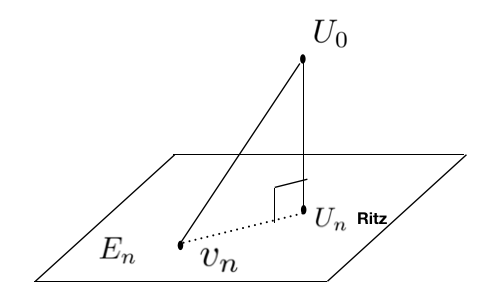
\includegraphics[width=0.5\linewidth]{Screen Shot 2024-03-14 at 16.38.30.png}
    \caption{}
    \label{fig:5}
\end{figure}


\section{Método de Galerkin}

Sean $\varphi_1,\ldots,\varphi_n,\ldots$ (base no necesariamente $\perp$ ) de $H_A$ y $\varphi_j \in D(A)$

consideremos el problema : $U_n = \sum\limits_{j=1}^n a_j \varphi_j$ 

\[
(A U_n -f, \varphi_k) = 0,\;\;\; k=1,\ldots n
\]

Si $U_n \overset{ H_n}{\rightarrow }  U_0$,  $A U_n \rightarrow f $, $A U_0 \rightarrow f $ 

\[ ( \sum\limits_j a_j A \varphi -f  , \varphi_k ) = 0 \]

\[  \sum\limits_j a_j (A\varphi_j, \varphi_k) = (f,\varphi_k) \]

Una proyección ortogonal $\perp_{\Vert\;\_A}$ sobre $E_n= U_n$ Ritz, este método se generaliza
al caso que $A$ no simétrico, $A$ no lineal, etc, ... si $U_n\rightarrow U_0$ en cierta norma.

\section{Sucesiones minimizantes}

\underline{Def:} $\{U_n\}\subset H_A$ es una sucesión minimizante si 

\[F(U_n)\rightarrow F(U_0) = \min F(U) \]

\begin{theorem}
    Si $\{ U_n\} $ es minimizante  $\Leftrightarrow \{ U_n\} \overset{H_A}{\rightarrow} U_0 $
\end{theorem}

\begin{proof}
    $"\Longleftarrow)"$ obvio
    $"\Rightarrow)"$ $F(U) = \Vert U- U_0\Vert_A^2 + F(U_0)$

    $F(U_n) \rightarrow F(U_0) \Rightarrow \Vert U_n-U_0\Vert_A \rightarrow 0$
    
\end{proof}

\begin{enumerate}
    \item \underline{Método de series ortogonales} 
    Sea $\varphi_1,\varphi_2, \ldots, \varphi_j \in H_A$ base ortonormal de $H_A$

    \[U_0= \sum\limits_{k=1}^\infty (U_0,\varphi_k)_A \varphi_k \]

    Sea $U_n = \sum_{k=1}^n (U_0 ,\varphi_k)_A \varphi_k $   depende de $U_0$ no conocido, proyección $\perp_{\Vert \;\;\Vert_A }$ sobre
    $\left< \varphi_1,\ldots,\varphi_n\right>$, $U_n\overset{H_A}{\rightarrow} U_0 $ 

    pero $(U,f)= (U, Kf)_A \Rightarrow (U_0,\varphi_k)_A = (f,\varphi_k)$

    $\Rightarrow U_n= \sum\limits_1^n (f,\varphi_k) \varphi_k$

    $U_0 = \sum\limits_1^\infty (f,\varphi_k)\varphi_k $ en general $\varphi_k$ no son $\perp$ en $H$

\section{Tarea}
\begin{figure}[H]
    \centering
    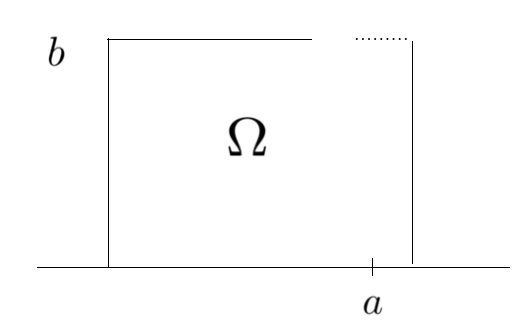
\includegraphics[width=0.5\linewidth]{Screen Shot 2024-03-14 at 18.49.42.png}
    \caption{}
    \label{fig:6}
\end{figure}

$A=-\Delta$, $H= L^2(\Omega)$, $D(A)= \{ U\in C^2 (\bar{\Omega}) , U|_{\partial \Omega} =0 \}$

Sea $\varphi_{n m}(x,y) = \sin \frac  {n \pi x}{ a}$ son completos en $L^2(\Omega)$ 

\begin{enumerate}
    \item Probar que $\varphi_{mn}$ son una base ortogonal en $H_A$
    \item Calcular la solución generalizada  de $-\Delta U = k= ct $  $U|_{\Omega}=0$

    \underline{Que problemas tiene} construcción de $\varphi_k$ base ortonormal en $H_A$

    sup.

    \[
    A= -\sum_{ i+j=2} a_{ij}(x,y) \frac{\partial^2}{ \partial _x^i  \partial _y^j}
    \]

    $a_{ij} = a_{ji}$, definida $>0$ elíptico
\end{enumerate}

\item \underline{Método de Ritz} Sea $\varphi_1,\ldots,\varphi_n,\ldots$ base (necesariamente ortogonal) de $H_A$

$\{ \varphi_1,\ldots,\varphi_n\}$ linealmente independientes

si $\{ \tilde{\varphi_1},\ldots,\tilde{\varphi_n\}}$ son $\perp_{\Vert \;\Vert_A}$ Gram-Schmidt son base $\perp_{\Vert \;\Vert_Aa}$ de $H_A$

Sea $E_n=\left< \varphi_1,\ldots,\varphi_n \right> = \left< \tilde{\varphi}_1,\ldots,\tilde{\varphi}_n \right>$

$v_n \in E_n : v_n = \sum\limits_1^n a_k \varphi_k = \sum\limits_1^n \tilde{a}_k \tilde{\varphi}_k$

\item \underline{Método de mínimos cuadrados}

Supongamos que $\varphi_1,\ldots,\varphi_n,\ldots \in D(A)$ y $A\varphi_1,\ldots,A\varphi_n,\ldots$ son una base (no necesariamente $\perp$) de $H$ 

Sea $AE_n= \{  \sum\limits_{k=1}^n a_k A\varphi_k \} \subset H$

Sea $f_n=$ proyección ortogonal de $f$ sobre $AE_n$

\[
f_n =\sum\limits_1^n a_k A \varphi_k 
\]

con $\Vert f-f_n\Vert$ mínima sobre $A E_n $

Sea $\hat{U}_n = \sum\limits_1^n a_k \varphi_k \in E_n$,  $A\hat{U}_n = f_n $
$\hat{ U}_n = K f_n \rightarrow Kf = U_0$ por continuidad de $K$

\begin{figure}[H]
    \centering
    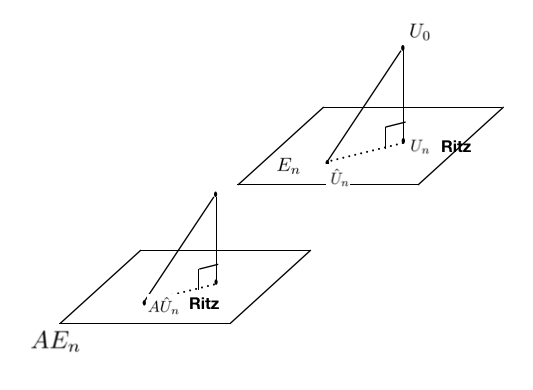
\includegraphics[width=0.5\linewidth]{Screen Shot 2024-03-17 at 18.25.51.png}
    \caption{}
    \label{fig:7}
\end{figure}

Nota: $\{ \varphi_1,\ldots, \varphi_n\}$ linealmente independientes en $H_A$, $\varphi_j\in D(A)$ $\Leftrightarrow$  $\{ A\varphi_1,\ldots, A\varphi_n\}$ 
linealmente independiente en $H$, $A \left( \sum\limits_1^n \lambda_i \varphi_i \right) =0 = \sum\limits_1^n A\varphi_i $ $A$ es $1-1$ 

\[\boxed{ \text{si } \{ A\varphi_1,\ldots, A\varphi_n\} \text{ es base de } H } \Rightarrow \boxed{ \{ \varphi_1,\ldots, \varphi_n\} \text{ es base de  } H_A} \]

$\varphi_1,\ldots,\varphi_n, \ldots $ base $\Leftrightarrow$ son linealmente independientes y $(U,\varphi)=0 \Rightarrow U=0$

$\tilde{\varphi}_1,\ldots,\tilde{\varphi}_n, \ldots $ $\perp$ Gram-Schmidth es base si 

\
\begin{enumerate}
    \item $(U,\tilde{\varphi}_j)=0 \Rightarrow U=0$
    \item $\Leftrightarrow (U,\varphi_j)=0$ 
\end{enumerate}

Si $(U,\varphi_j)_A =0$  $U\in H_A \subset H$ 

$(U,A\varphi_j)=0 \Rightarrow U=0$

AL REVES

$\varphi_1,\ldots$ base de $H_A$ $\varphi_j\in D(A) $  $\nRightarrow $  $A\varphi_j$ base de $H$

$A$ simétrico $(AU,U)\geq c \Vert U\Vert^2$

$\Vert U\Vert_A^2 = \underset{n\rightarrow\infty }{\lim} (AU_n,U_n)$  $\left( \Vert U\Vert_A^2 =\iint_\Omega |\nabla U|^2\right)$

$U_n \in D(A) $ Cauchy en $\Vert \;\Vert_A$

$H_A= \widehat{D(A)}^{\Vert\;\Vert_A} $  $H_A=H_0^1$

$F(U) = \Vert U \Vert_A^2 -2 (f,U) = \Vert U-U_0 \Vert_A^2 + \Vert U_0\Vert_A^2$

tiene un \underline{único} mínimo $U_0$ sobre $H_A$

\begin{figure}[H]
    \centering
    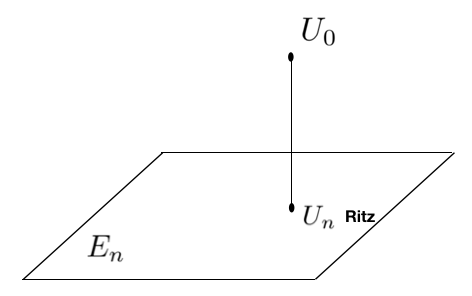
\includegraphics[width=0.5\linewidth]{Screen Shot 2024-03-26 at 09.44.11.png}
    \caption{Enter Caption}
    \label{fig:8}
\end{figure}

$\varphi_1, \varphi_2 , \ldots $ base de $H_A$

$E_n = < \varphi_1, \ldots,\varphi_n >  $

$F|_{E_n}$ tiene mínimo en $U_n$ Ritz

$U_n= \sum\limits_1^n a_j \varphi_j $

Galerkin 

$(AU_n-f_j,\varphi_j)=0  \;j=1,\ldots,n$  $\varphi_j\in D(A)$

$ A_n \left(  \begin{array}{c}
a_1\\
\vdots\\
a_n
\end{array}
\right) = B_n $

\underline{Mínimos cuadrados}

$\varphi_1,\varphi_2,\ldots\in D(A)$ $\{ A \varphi_j \}$ base de $H\Rightarrow \{ \varphi_j\}$ base de $H_A$

\begin{figure}
    \centering
    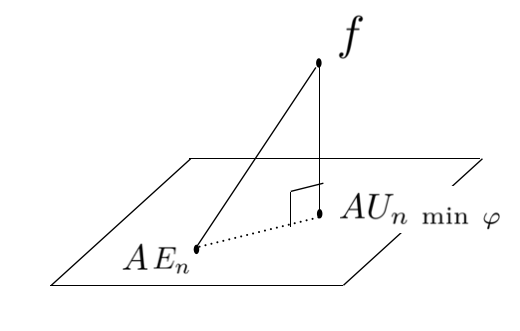
\includegraphics[width=0.5\linewidth]{Screen Shot 2024-03-26 at 19.24.50.png}
    \caption{Enter Caption}
    \label{fig:9}
\end{figure}

$\min \Vert f- A U_n \Vert^2$

$C_n \left( 
\begin{array}{c}
     a_1  \\
     \vdots\\
     a_n
\end{array}
\right)= D_n$

$(C_n)_{ij}= (A\varphi_i,A\varphi_j)$ 

$(D_n)_{ij}= (A\varphi_i,f)$

Teoricamente

$\Vert U_0-U_{n\;Ritz}\Vert_A \leq \Vert U_0 - U_{n\;min\;\varphi} \Vert_A $

$\Vert \underset{ \overset{||}{Kf} }{U_0}  -U_{n\;min\;\varphi}\Vert_A \leq \frac{1}{\sqrt{c}} \Vert A U_{n\;\min\;\varphi } -f\Vert$

$t A U_{n\;\min\;\varphi } -f$ si es medible

\item Método de Courant (o de penalización) 

$\varphi_{1},\varphi_{2},\ldots\in D(A)$  $\{A\varphi_j \}$ base de $H$

\begin{figure}[H]
    \centering
    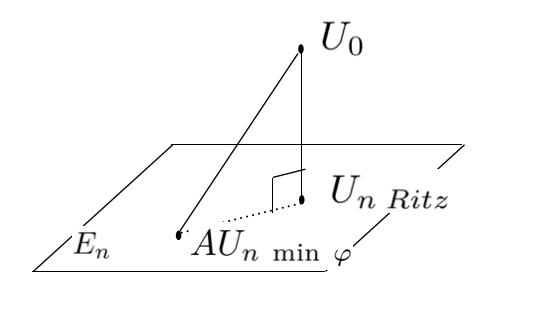
\includegraphics[width=0.5\linewidth]{Screen Shot 2024-03-26 at 19.35.32.png}
    \caption{Método de Courant}
    \label{fig:10}
\end{figure}

Suponemos que $U_0\in D(A) \Rightarrow AU_0 = f$ 

defino un nuevo funcional 

Sea
\[
\tilde{F}(U)= F(U) + \Vert AU -f \Vert^2  
\]


definido sobre $D(A) \subset H_A \subset H$

\[
\tilde{F}(U) \geq F(U) \geq F(U_0)
\]

\[
\tilde{F}(U_0) = F(U_0)
\]

puedo decir que $U_0$ es mínimo de $\tilde{F}$ 

sea $\tilde{F}|_{E_n}$ es una forma cuadrática acotada por abajo $\Rightarrow$ mínimo talque 
$\frac{\partial \tilde{F}}{\partial a_j} =0$. Para ver que es único hago lo siguiente

$\tilde{F}(U) = \Vert U -U_0\Vert_A^2 + \Vert A U-f \Vert^2 -\Vert U_0\Vert^2$ 

$\Vert v-U\Vert_A^2 = 2 \left( \Vert v-U_0 \Vert_A^2 +\Vert U-U_0\Vert_A^2 - \Vert U_0 -\frac{U+v}{2}\Vert_A^2  \right)$

$\Vert Av -AU\Vert^2= 2\left(  \Vert  Av-f\Vert^2 + \Vert AU-f\Vert^2  - 2 \Vert f - \frac{A(U+v)}{2} \Vert^2\right)$

 $\Rightarrow$  
 \[
 \Vert v-U\Vert^2 + \Vert A (v-U)\Vert^2 = 2 \left( \tilde{F}(v) + \Vert U_0\Vert_A^2 + \tilde{F}(U) + \Vert U_0\Vert_A^2 - 2\tilde{F}\left( \frac{U+v}{2} \right) - 2 \Vert U_0\Vert_A^2 \right)  \]

si $U,v \in E_n $ con $\tilde{F}(U)= \tilde{F}(v) = \underset{E_n}{\min} \tilde{F} = d_n$

\[
 \Vert v-U\Vert^2 + \Vert A (v-U)\Vert^2 = 4\left( d_n - \tilde{F} \left(\frac{U+v}{2} \right) \right)\leq 0 
\]

$\Rightarrow$ mínimo único


Si $U= \sum\limits_j^n a_j \varphi_j $   $AU = \sum\limits_j^n a_j A \varphi_j$

\[
\frac{\partial \tilde{F}}{ \partial a_j } = 2 \sum\limits_{i=1}^n a_j (\varphi_i,f_j)_A
\]
  \end{enumerate}

 \end{document}